%%%%%%%%%%%%%%%%%%%%%%%%%%%%%%%%%%%%%%%%%%%%%%%%%%%%%%%%%%%%%%%%%%%%%
%%   APPENDIX: Extra details that are too long or ugly for main part of book
%%%%%%%%%%%%%%%%%%%%%%%%%%%%%%%%%%%%%%%%%%%%%%%%%%%%%%%%%%%%%%%%%%%%%

\renewcommand{\chapterfolder}{glider_synthesis/}
\chapterimage{cover/appendix_extra}

\chapter{Extra Details}\label{chp:appendix_extras}

In this appendix, we provide some details that makes theorems or pattern from the main text more precise, but whose details are so long, ugly, or technical that we prefer to hide them away.

%% http://conwaylife.com/forums/viewtopic.php?f=2&t=299
%% http://conwaylife.com/forums/viewtopic.php?f=2&t=1512&start=50
\section{Universality of the Clock Inserter}\label{chp:appendix_salvo}

In Section~\ref{sec:slow_salvo}, we showed that we can use a p1 slow salvo to simulate any glider synthesis in which the gliders are not ``too close'' together, and we suggested that the clock inserter\index{clock!inserter} from Figure~\ref{fig:clock_inserter} could be used to remove that final spacing restriction. Here we demonstrate the nitty-gritty details needed to show that the clock inserter really can create any tight packing of gliders that we desire, thus showing that \emph{all} glider syntheses can be implemented via a p1 slow salvo.


\subsection{Timing of Tight Glider Salvos}\label{sec:salvo_timing}

Recall the definitions of glider lanes and timing from Section~\ref{sec:glider_lanes}, which give us a way to discuss how close gliders are to each other in both perpendicular directions. We now investigate exactly how tightly gliders in a salvo can be packed. For example, we mentioned in Section~\ref{sec:glider_loops} that two gliders in the same lane must be at least $14$ generations apart from each other or else they will collide. Similarly, it is straightforward to check that gliders that differ by $0, 1, 2, 3, 4, 5,$ or $6$ lanes must have their timings offset by at least $14, 14, 14, 13, 11, 9,$ or $7$ generations, respectively, as demonstrated in Figure~\ref{fig:tight_glider_packings}. On the other hand, gliders that differ by $7$ lanes or more will never collide with each other, regardless of their timings, since the Moore neighbourhoods of those lanes do not overlap enough to cause an unexpected birth between the gliders.

\begin{figure}[!htb]
	\centering
	\patternimglinkwidth{\textwidth}{tight_glider_packings}
	\caption{The closest timings that are possible between two gliders in nearby lanes without colliding with each other. From left to right, these gliders differ by $0, 1, 2, 3, 4, 5,$ and $6$ lanes, and their timings differ by $14, 14, 14, 13, 11, 9,$ and $7$ generations. The rightmost image shows that gliders that differ by $7$ lanes can never collide with each other.}\label{fig:tight_glider_packings}
\end{figure}


\subsection{Timing of the Clock Inserter}\label{sec:clock_inserter_timing}

The basic idea behind proving universality of the clock inserter is to show that we can use it to place gliders next to each other in each of the tight configurations from Figure~\ref{fig:tight_glider_packings}. However, this alone is not enough to prove the theorem, since a glider salvo might have dozens of tightly-packed gliders, and a priori it's not obvious that being able to place any pair of gliders means that we can place any complicated configuration of multiple gliders---it could be that no matter which order we place the gliders pairs in, we eventually get blocked off from placing one of the gliders that has other gliders on all sides of it.

To get around this problem, we establish a precise ordering that we will use to construct the salvo. Since the clock inserter is good at placing a glider closely in front of another glider, but bad at placing a glider closely behind another glider, we build the salvo from back-to-front. Specifically, we say that a glider's \textbf{rank} is its lane number plus its timing (see Figure~\ref{fig:glider_ranks}), and we construct the salvo in order from the lowest-ranked glider to the highest-ranked glider (breaking ties arbitrarily).\footnote{While the lane and timing of a glider are concepts that are regularly used in the Life community, we have introduced the rank of a glider very specifically for this proof.}

\begin{figure}[!ht]
	\centering
	\gridbox{0.75pt}{\begin{tikzpicture}[scale=0.5, every node/.style={transform shape}]%
		\node[inner sep=0pt,anchor=south west] (glider_loop) at (0.5,0.5) {\patternimgwidth{7cm}{glider_slope_chart_c}};
		
		\letternode{1}{1}{-9}
		\letternode{2}{1}{-6}
		\letternode{3}{1}{-3}
		\letternode{4}{1}{0}
		\letternode{5}{1}{3}
		\letternode{6}{1}{6}
		\letternode{7}{1}{9}
		
		\letternode{1}{2}{$\cdot$}
		\letternode{2}{2}{-7}
		%\letternode{3}{2}{-4}
		%\letternode{4}{2}{-1}
		\letternode{5}{2}{2}
		\letternode{6}{2}{5}
		\letternode{7}{2}{8}
		
		\letternode{1}{3}{$\cdot$}
		%\letternode{2}{3}{-8}
		\letternode{3}{3}{-5}
		%\letternode{4}{3}{-2}
		\letternode{5}{3}{1}
		\letternode{6}{3}{4}
		\letternode{7}{3}{7}
		
		\letternode{1}{4}{$\cdot$}
		\letternode{2}{4}{-9}
		\letternode{3}{4}{-6}
		%\letternode{4}{4}{-3}
		\letternode{5}{4}{0}
		\letternode{6}{4}{3}
		\letternode{7}{4}{6}
		
		\letternode{1}{5}{$\cdot$}
		\letternode{2}{5}{$\cdot$}
		\letternode{3}{5}{-7}
		\letternode{4}{5}{-4}
		\letternode{5}{5}{-1}
		\letternode{6}{5}{2}
		\letternode{7}{5}{5}
		
		\letternode{1}{6}{$\cdot$}
		\letternode{2}{6}{$\cdot$}
		\letternode{3}{6}{-8}
		\letternode{4}{6}{-5}
		\letternode{5}{6}{-2}
		\letternode{6}{6}{1}
		\letternode{7}{6}{4}
		
		\letternode{1}{7}{$\cdot$}
		\letternode{2}{7}{$\cdot$}
		\letternode{3}{7}{-9}
		%\letternode{4}{7}{-6}
		%\letternode{5}{7}{-3}
		%\letternode{6}{7}{0}
		\letternode{7}{7}{3}
		
		\letternode{1}{8}{$\cdot$}
		\letternode{2}{8}{$\cdot$}
		\letternode{3}{8}{$\cdot$}
		\letternode{4}{8}{-7}
		\letternode{5}{8}{-4}
		%\letternode{6}{8}{-1}
		\letternode{7}{8}{2}
		
		\letternode{1}{9}{$\cdot$}
		\letternode{2}{9}{$\cdot$}
		\letternode{3}{9}{$\cdot$}
		\letternode{4}{9}{-8}
		%\letternode{5}{9}{-5}
		\letternode{6}{9}{-2}
		\letternode{7}{9}{1}
		
		\letternode{1}{10}{$\cdot$}
		\letternode{2}{10}{$\cdot$}
		\letternode{3}{10}{$\cdot$}
		\letternode{4}{10}{-9}
		\letternode{5}{10}{-6}
		\letternode{6}{10}{-3}
		\letternode{7}{10}{0}
		
		\end{tikzpicture}}
	\caption{Two gliders that both have a rank of~$0$. The numbers displayed on the grid show the rank of a glider when its leading cell (in the phase of the glider at the top) is at that location. The glider at the bottom has rank $0$ since it will be in that phase in $2$ generations, and its leading cell in that phase will be at a location labelled ``$2$''. Rank increases by $3$ every cell to the right and by $1$ every cell down, so gliders with constant rank lie on lines of slope $3$ in the Life plane.}\label{fig:glider_ranks}
\end{figure}

We need to show that if we insert gliders into the salvo according to their rank, then the (already-placed) low-rank gliders do not collide with the clock inserter reaction as we place the high-rank gliders. To this end, suppose that the glider we are inserting via the clock inserter is in lane $0$ and has timing $0$ (and thus rank~$0$). We will prove the result by contradiction, so let's assume that there is a glider in the salvo that has already been placed that collides with the clock inserter reaction. We derive the contradiction by splitting into two cases, based on the lane of the glider that collides with the clock inserter. Note that all lane and timing (and thus hence rank) numbers that we describe for this interfering glider are relative to the rank $0$ glider that we are inserting. \\

\noindent \textbf{Case 1:} The colliding glider is in one of the lanes $-6, -5, \ldots, 5, 6$.

If the timing of the glider in a particular lane is small enough (i.e., far enough below $0$), it will be far to the top-left of the clock inserter reaction and thus not collide with it. It is straightforward (albeit somewhat tedious) to calculate the smallest possible timing of a glider in each lane $-6, -5, \ldots, 5, 6$ that \emph{does} collide with the clock inserter, and these values are presented in Table~\ref{tab:clock_inserter_ranks}.

\begin{table}[!htb]
	\begin{center}		
		\begin{tabular}{r c c c c c c c}
			\toprule
			Lane: & $0$ & $1$ & $2$ & $3$ & $4$ & $5$ & $6$ \\
			\rowcolor{gray!20} Min. timing: & $-13$ & $-13$ & $-13$ & $-12$ & $-10$ & $-8$ & $-6$ \\\bottomrule
		\end{tabular}
		\caption{The minimal timing that a glider in lanes $0$ through $6$ can have if it collides with the clock inserter reaction. The minimal timing for a glider in lane $-n$ in all of these cases is the same as the timing for a glider in lane $n$.}\label{tab:clock_inserter_ranks}
	\end{center}
\end{table}

Since any pair of gliders with timing differences as in Table~\ref{tab:clock_inserter_ranks} would also collide with each other (refer back to the timings listed in Figure~\ref{fig:tight_glider_packings}), we conclude that if a glider in one of these lanes collides with the clock inserter, then it would also collide with the output glider and thus those two gliders could not be part of the same salvo in the first place. \\

\noindent \textbf{Case 2:} The colliding glider is in one of the lanes $\ldots, -9, -8, -7$ or $7, 8, 9, \ldots$.

In a similar vein to that of case~1, we can calculate the minimum possible timing (and thus minimum rank) of a glider that collides with the clock inserter in each of these lanes, and these values are presented in Table~\ref{tab:clock_inserter_ranks_b}. In this case, however, we are interested in the rank of the colliding glider rather than its timing, and we notice that in each case, regardless of the glider's lane, its rank is strictly positive, which contradicts the fact that we are inserting gliders in order of increasing rank, and we are currently inserting a glider with rank $0$.

\begin{table}[!htb]
	\begin{center}		
		\begin{tabular}{r c c c c c c | c c c c c c}
			\toprule
			Lane: & $-n$ & $-11$ & $-10$ & $-9$ & $-8$ & $-7$ & $7$ & $8$ & $9$ & $10$ & $11$ & $n$ \\
			\rowcolor{gray!20} Min. timing: & $2n-5$ & $17$ & $15$ & $13$ & $11$ & $9$ & $-3$ & $15$ & $17$ & $19$ & $21$ & $2n-1$ \\
			Min. rank: & $n-5$ & $6$ & $5$ & $4$ & $3$ & $2$ & $4$ & $23$ & $26$ & $29$ & $32$ & $3n-1$ \\\bottomrule
		\end{tabular}
		\caption{The smallest possible timing and rank that a glider in lanes $\ldots, -9, -8, -7$ or $7, 8, 9, \ldots$ can have if they collide with the clock inserter reaction. Importantly, the rank of the colliding glider is positive in all cases.}\label{tab:clock_inserter_ranks_b}
	\end{center}
\end{table}

While this contradiction completes the proof of universality of the clock inserter, it is worth focusing on some of the values in Table~\ref{tab:clock_inserter_ranks_b} and clarifying some points about the rank of a glider:\smallskip

\begin{itemize}
	\item First, the obvious pattern in Table~\ref{tab:clock_inserter_ranks} of the minimal timing increasing by $2$ generations every time the glider moves farther out by $1$ lane does indeed continue forever---the collision that happens in these lanes occurs with one of the input gliders to the clock inserter rather than with the clock itself, which explains the regular pattern.\smallskip
	
	\item Second, lane~7 is somewhat of an anomaly in Table~\ref{tab:clock_inserter_ranks_b}, with the minimal timing of the glider in that lane being much lower than in the other lanes. The reason for this oddity is that the clock in the clock inserter sticks one lane farther to the right the output glider does, which causes early collisions in this lane, and this lane only. This minimum-timing lane-7 glider collision is displayed in Figure~\ref{fig:clock_inserter_7_lanes}.\smallskip
\end{itemize}

\begin{figure}[!htb]
	\centering
	\begin{subfigure}{.43\textwidth}
		\centering\embedlink{clock_inserter_7_lanes_ok}{\vcenteredhbox{\patternimg{0.12}{clock_inserter_7_lanes_ok}} \vcenteredhbox{\genarrow{12}} \vcenteredhbox{\patternimg{0.12}{clock_inserter_7_lanes_ok_12}}}
		\caption{Lane $7$, timing $-4$.}\label{fig:clock_inserter_7_lanes_ok}
	\end{subfigure} \ \ \ \ % 
	\begin{subfigure}{.53\textwidth}
		\centering\embedlink{clock_inserter_7_lanes_bad}{\vcenteredhbox{\patternimg{0.12}{clock_inserter_7_lanes_bad}} \vcenteredhbox{\genarrow{6}} \vcenteredhbox{\patternimg{0.12}{clock_inserter_7_lanes_bad_6}} \vcenteredhbox{\genarrow{1}} \vcenteredhbox{\patternimg{0.12}{clock_inserter_7_lanes_bad_7}}}
		\caption{Lane $7$, timing $-3$.}\label{fig:clock_inserter_7_lanes_bad}
	\end{subfigure}
	\caption{A clock inserter attempting to insert a glider in lane $0$ at timing $0$ when there is already a glider in lane 7 with (a)~timing $-4$ and (b)~timing $-3$. In (a), the new glider is successfully inserted, but in (b), a cell from the clock (shown in \bgbox{greenback}{green} in generation 6) interferes with the glider from lane~7, causing an extra cell to be born (shown in \bgbox{orangeback}{orange} in generation 7).}\label{fig:clock_inserter_7_lanes}
\end{figure}

In fact, the anomaly in lane~7 is exactly why we insert gliders according to their rank rather than (for example) their timing. If we inserted gliders in order from low timing to high timing (i.e., according to diagonal lines of slope $1$ in the Life plane) then we can run into problems when trying to insert gliders that are $7$ lanes apart from each other. However, our choice of defining a glider's rank to equal its lane number plus its timing is by no means the only way of ranking gliders that works. Many other choices are possible, and each ranking function corresponds to lines of different slopes in the Life plane (see Exercise~\ref{exer:slow_salvo_clock_slope}).


\renewcommand{\chapterfolder}{universal_construction/}
%%%%%%%%%%%%%%%%%%%%%%%%%%%%%%%%
\section{Snarkmaker Timings}\label{sec:appendix_snarkmaker}
%%%%%%%%%%%%%%%%%%%%%%%%%%%%%%%%

In Section~\ref{sec:snarkmaker_itself}, we described how to build a single-channel recipe called a Snarkmaker\index{Snarkmaker} that constructs a Snark along its path, while simultaneously moving the construction elbow to its far side. This recipe consists of $2{\thousep}427$ gliders (specified by $2{\thousep}426$ glider spacings), and is presented here:\\[-0.1cm]

\begin{sloppypar}
	\noindent\tiny\texttt{109, 91, 93, 90, 132, 115, 127, 91, 90, 91, 95, 90, 114, 162, 233, 159, 90, 155, 126, 93, 118, 90, 91, 90, 1000, 109, 91, 94, 91, 91, 92, 90, 169, 91, 90, 116, 90, 113, 1000, 109, 91, 93, 91, 156, 91, 91, 94, 90, 91, 140, 91, 103, 91, 91, 132, 1000, 109, 90, 93, 91, 91, 90, 90, 100, 90, 90, 146, 96, 90, 90, 90, 92, 156, 144, 1000, 109, 91, 93, 91, 132, 115, 102, 90, 91, 91, 91, 90, 90, 154, 1000, 93, 91, 118, 91, 151, 90, 159, 91, 92, 90, 136, 90, 90, 154, 90, 101, 104, 165, 129, 91, 109, 91, 93, 91, 97, 90, 91, 111, 91, 116, 91, 94, 330, 91, 90, 95, 91, 90, 90, 91, 123, 90, 91, 152, 90, 90, 93, 91, 116, 91, 131, 91, 95, 188, 113, 91, 91, 147, 122, 91, 173, 91, 91, 133, 247, 92, 90, 109, 91, 93, 91, 129, 148, 91, 93, 154, 90, 134, 91, 91, 90, 91, 91, 111, 91, 91, 91, 91, 91, 109, 90, 93, 91, 91, 158, 94, 113, 91, 90, 91, 96, 90, 142, 91, 109, 91, 94, 91, 91, 179, 91, 90, 94, 91, 114, 90, 166, 90, 90, 90, 91, 117, 90, 96, 90, 90, 95, 91, 91, 109, 91, 93, 90, 156, 91, 91, 94, 91, 90, 147, 117, 91, 144, 90, 91, 128, 100, 91, 90, 105, 91, 91, 109, 91, 94, 91, 91, 124, 91, 105, 90, 169, 91, 90, 116, 91, 142, 90, 90, 91, 109, 91, 93, 91, 92, 91, 90, 90, 95, 102, 91, 91, 91, 130, 91, 90, 136, 91, 91, 119, 113, 90, 91, 114, 90, 109, 91, 94, 91, 91, 179, 91, 90, 94, 91, 102, 91, 151, 90, 90, 101, 90, 91, 125, 184, 90, 90, 90, 109, 91, 94, 91, 91, 179, 91, 90, 94, 91, 102, 91, 151, 90, 90, 101, 90, 91, 125, 184, 90, 90, 90, 109, 91, 93, 90, 140, 150, 132, 212, 103, 90, 98, 90, 148, 90, 90, 91, 91, 91, 119, 101, 108, 90, 91, 91, 119, 90, 109, 91, 94, 91, 90, 99, 90, 112, 90, 91, 105, 90, 121, 118, 103, 90, 144, 117, 95, 91, 109, 91, 93, 91, 92, 91, 90, 90, 95, 102, 91, 91, 91, 130, 91, 90, 136, 91, 91, 119, 113, 90, 91, 114, 91, 109, 90, 93, 91, 91, 181, 90, 95, 110, 114, 100, 160, 90, 143, 91, 119, 90, 106, 129, 109, 91, 93, 91, 92, 91, 90, 90, 162, 91, 91, 90, 129, 91, 113, 90, 90, 90, 90, 109, 91, 93, 90, 140, 150, 142, 91, 90, 111, 91, 91, 193, 97, 91, 91, 155, 90, 98, 90, 91, 93, 91, 151, 90, 139, 180, 103, 115, 167, 91, 120, 139, 135, 91, 91, 170, 109, 91, 93, 90, 155, 106, 91, 121, 90, 90, 91, 137, 90, 232, 90, 91, 91, 94, 90, 171, 90, 91, 103, 102, 109, 91, 93, 91, 137, 90, 166, 91, 102, 90, 104, 91, 96, 96, 91, 90, 90, 90, 166, 90, 90, 93, 90, 91, 109, 91, 94, 91, 91, 124, 91, 105, 91, 119, 91, 132, 99, 90, 90, 90, 150, 160, 116, 91, 91, 91, 90, 96, 90, 90, 109, 91, 93, 90, 171, 90, 90, 91, 90, 91, 90, 91, 129, 144, 90, 90, 120, 90, 91, 91, 169, 90, 91, 109, 91, 93, 91, 118, 90, 91, 91, 91, 104, 219, 91, 135, 105, 154, 90, 91, 164, 91, 132, 90, 90, 140, 94, 93, 90, 96, 90, 90, 91, 149, 90, 90, 161, 100, 109, 91, 93, 91, 92, 91, 90, 90, 124, 91, 142, 90, 90, 91, 91, 112, 90, 102, 102, 103, 90, 90, 90, 117, 112, 90, 189, 90, 90, 109, 91, 93, 91, 92, 91, 90, 90, 162, 91, 91, 90, 129, 91, 113, 90, 90, 90, 90, 109, 91, 93, 91, 92, 90, 97, 91, 116, 91, 145, 90, 91, 98, 90, 90, 188, 91, 91, 91, 90, 115, 91, 109, 91, 93, 91, 97, 91, 90, 91, 120, 91, 117, 91, 123, 90, 118, 91, 146, 110, 160, 90, 109, 91, 93, 90, 129, 148, 90, 93, 90, 143, 96, 92, 90, 165, 90, 118, 90, 90, 91, 91, 109, 91, 94, 91, 91, 93, 90, 158, 90, 91, 90, 90, 116, 104, 109, 91, 94, 91, 91, 167, 90, 90, 91, 95, 90, 90, 148, 90, 151, 90, 90, 136, 134, 155, 115, 103, 91, 109, 91, 93, 90, 155, 106, 91, 121, 90, 90, 91, 137, 90, 232, 90, 91, 91, 94, 90, 171, 90, 91, 103, 101, 109, 91, 94, 91, 91, 136, 91, 91, 90, 168, 90, 90, 110, 90, 90, 93, 91, 111, 91, 91, 90, 132, 91, 91, 93, 91, 118, 90, 137, 91, 173, 93, 158, 90, 90, 90, 118, 90, 91, 90, 151, 154, 167, 91, 133, 90, 119, 178, 155, 90, 90, 90, 109, 91, 94, 91, 91, 95, 91, 90, 93, 218, 142, 90, 91, 161, 90, 138, 90, 162, 91, 90, 140, 95, 109, 109, 91, 93, 91, 92, 91, 98, 201, 91, 129, 90, 90, 90, 90, 90, 103, 90, 108, 90, 104, 90, 109, 91, 93, 90, 129, 148, 90, 93, 90, 143, 96, 92, 90, 165, 90, 118, 90, 90, 91, 91, 109, 91, 94, 91, 91, 179, 91, 90, 94, 91, 111, 90, 90, 90, 171, 91, 110, 91, 154, 90, 132, 91, 109, 91, 94, 91, 91, 124, 90, 144, 90, 90, 90, 165, 119, 90, 104, 90, 100, 90, 90, 91, 109, 91, 93, 91, 92, 91, 90, 90, 162, 91, 91, 90, 129, 91, 113, 90, 90, 90, 91, 109, 91, 94, 91, 91, 95, 91, 90, 93, 218, 172, 90, 90, 90, 116, 112, 341, 107, 106, 90, 163, 91, 90, 109, 91, 93, 90, 169, 90, 91, 103, 91, 133, 90, 90, 91, 91, 90, 110, 91, 93, 90, 112, 171, 90, 109, 91, 94, 91, 91, 171, 91, 90, 113, 90, 97, 114, 90, 105, 90, 139, 90, 113, 90, 106, 98, 121, 90, 109, 91, 94, 91, 91, 124, 90, 142, 90, 90, 146, 91, 153, 90, 102, 91, 152, 108, 97, 91, 109, 91, 94, 91, 91, 124, 90, 170, 90, 90, 91, 90, 99, 91, 90, 91, 110, 121, 161, 117, 115, 137, 90, 91, 90, 109, 90, 93, 91, 91, 128, 90, 139, 91, 90, 97, 91, 124, 157, 91, 90, 90, 129, 144, 91, 91, 147, 130, 91, 90, 90, 91, 90, 140, 90, 92, 90, 90, 109, 91, 93, 90, 156, 91, 91, 102, 91, 91, 90, 90, 106, 91, 166, 90, 125, 91, 90, 126, 91, 109, 91, 94, 91, 91, 179, 91, 90, 94, 91, 102, 91, 151, 90, 90, 101, 90, 91, 125, 184, 90, 90, 90, 93, 91, 151, 90, 139, 180, 103, 115, 167, 91, 120, 139, 135, 91, 91, 170, 109, 90, 93, 91, 91, 128, 90, 139, 91, 90, 97, 91, 124, 157, 91, 90, 90, 129, 144, 91, 91, 147, 130, 91, 90, 90, 91, 90, 140, 90, 92, 90, 90, 109, 91, 93, 91, 145, 215, 114, 91, 121, 91, 150, 91, 91, 153, 91, 141, 90, 91, 91, 90, 123, 91, 109, 90, 101, 169, 213, 133, 195, 90, 132, 143, 91, 139, 138, 158, 151, 99, 91, 108, 99, 91, 90, 91, 91, 90, 91, 131, 91, 109, 91, 93, 90, 156, 91, 91, 96, 132, 91, 91, 106, 91, 90, 119, 185, 91, 96, 90, 132, 90, 91, 90, 142, 109, 91, 94, 91, 91, 124, 90, 170, 90, 90, 91, 90, 99, 91, 90, 91, 110, 121, 161, 117, 115, 137, 90, 91, 90, 109, 91, 93, 90, 155, 106, 91, 121, 90, 90, 91, 137, 90, 232, 90, 91, 91, 94, 90, 171, 90, 91, 103, 102, 109, 91, 93, 90, 129, 148, 91, 102, 91, 91, 145, 178, 91, 115, 90, 90, 91, 104, 90, 90, 92, 249, 90, 90, 91, 109, 91, 94, 91, 90, 152, 91, 90, 91, 117, 90, 91, 111, 91, 91, 118, 90, 145, 90, 100, 116, 90, 90, 99, 90, 109, 91, 94, 91, 91, 128, 126, 90, 161, 151, 90, 109, 91, 90, 90, 94, 144, 106, 90, 94, 90, 90, 90, 109, 91, 94, 91, 91, 124, 91, 105, 90, 169, 91, 90, 116, 91, 142, 90, 90, 91, 109, 91, 93, 90, 140, 150, 108, 91, 90, 111, 91, 91, 194, 98, 90, 169, 90, 109, 91, 94, 91, 91, 141, 90, 171, 90, 155, 90, 111, 91, 90, 130, 90, 91, 90, 97, 90, 90, 109, 91, 94, 91, 91, 121, 90, 90, 90, 90, 90, 90, 99, 90, 165, 119, 90, 106, 90, 90, 91, 109, 91, 94, 91, 91, 93, 90, 95, 90, 113, 90, 99, 90, 156, 90, 90, 90, 138, 170, 109, 91, 94, 91, 91, 92, 90, 169, 90, 90, 90, 107, 90, 90, 91, 90, 95, 91, 91, 109, 91, 93, 90, 171, 90, 90, 91, 90, 91, 90, 91, 129, 144, 90, 90, 120, 90, 91, 91, 169, 90, 91, 109, 90, 95, 245, 90, 131, 135, 90, 90, 154, 90, 91, 91, 91, 111, 90, 90, 91, 91, 128, 91, 96, 91, 109, 91, 94, 91, 91, 124, 91, 105, 91, 119, 91, 132, 99, 90, 90, 90, 150, 160, 116, 91, 91, 91, 90, 96, 90, 91, 93, 91, 116, 91, 151, 90, 109, 111, 127, 91, 113, 91, 169, 186, 90, 90, 158, 91, 90, 90, 90, 117, 91, 160, 90, 91, 96, 90, 90, 91, 109, 91, 94, 91, 90, 95, 91, 90, 147, 167, 90, 160, 90, 160, 104, 90, 90, 91, 91, 101, 139, 91, 90, 136, 129, 90, 109, 91, 93, 91, 123, 91, 118, 90, 91, 108, 91, 91, 90, 90, 90, 90, 143, 91, 92, 177, 129, 101, 167, 91, 90, 90, 91, 130, 127, 90, 137, 91, 93, 90, 91, 91, 94, 229, 107, 91, 90, 104, 91, 91, 101, 91, 91, 93, 90, 119, 90, 133, 90, 91, 93, 145, 91, 132, 91, 109, 91, 93, 91, 137, 90, 166, 91, 102, 90, 104, 91, 96, 96, 91, 90, 90, 90, 166, 90, 90, 93, 90, 90, 109, 90, 93, 91, 91, 128, 90, 139, 91, 90, 97, 91, 124, 157, 91, 90, 90, 129, 144, 91, 91, 147, 130, 91, 90, 90, 91, 90, 140, 90, 92, 90, 91, 123, 270, 90, 125, 90, 90, 90, 94, 137, 123, 90, 145, 136, 90, 91, 100, 91, 105, 91, 153, 91, 90, 145, 155, 109, 91, 93, 91, 92, 91, 139, 90, 91, 91, 90, 96, 130, 97, 91, 164, 90, 97, 91, 90, 91, 114, 90, 90, 118, 90, 90, 123, 270, 90, 125, 90, 90, 90, 94, 137, 123, 90, 145, 136, 90, 91, 100, 91, 105, 91, 153, 91, 90, 145, 155, 109, 90, 93, 91, 91, 148, 91, 90, 151, 90, 91, 163, 108, 151, 112, 144, 90, 149, 90, 90, 99, 90, 109, 91, 94, 91, 91, 124, 91, 126, 91, 140, 162, 148, 90, 90, 119, 90, 91, 109, 91, 93, 91, 155, 106, 91, 91, 96, 90, 90, 91, 108, 90, 156, 90, 90, 120, 90, 112, 91, 99, 91, 109, 91, 93, 91, 129, 148, 91, 93, 154, 90, 134, 91, 91, 90, 91, 91, 111, 91, 91, 91, 91, 90, 109, 91, 93, 91, 129, 148, 91, 93, 154, 90, 134, 91, 91, 90, 91, 91, 111, 91, 91, 91, 91, 90, 109, 91, 93, 91, 129, 149, 91, 90, 90, 142, 219, 90, 99, 91, 109, 115, 92, 185, 91, 109, 90, 93, 91, 91, 142, 90, 98, 90, 91, 125, 114, 127, 90, 111, 90, 109, 91, 93, 91, 130, 91, 90, 134, 90, 90, 103, 122, 156, 112, 90, 183, 117, 91, 152, 141, 90, 98, 90, 91, 93, 91, 116, 91, 131, 91, 95, 188, 113, 91, 91, 147, 122, 91, 173, 91, 91, 133, 247, 92, 91, 109, 91, 93, 90, 156, 91, 91, 94, 91, 90, 147, 117, 91, 144, 90, 91, 128, 100, 91, 90, 105, 91, 91, 93, 91, 116, 91, 106, 91, 155, 90, 106, 90, 167, 90, 90, 91, 148, 123, 111, 155, 91, 105, 90, 90, 92, 90, 124, 90, 91, 109, 91, 94, 91, 91, 95, 91, 90, 97, 143, 171, 90, 105, 90, 91, 144, 91, 90, 90, 90, 94, 90, 90, 90, 109, 91, 93, 91, 92, 90, 158, 90, 94, 270, 172, 130, 90, 91, 91, 96, 90, 90, 147, 91, 109, 91, 93, 91, 92, 90, 162, 90, 129, 91, 91, 91, 90, 137, 99, 90, 90, 111, 91, 153, 90, 90, 90, 109, 91, 95, 125, 128, 90, 90, 90, 172, 90, 90, 90, 119, 91, 113, 247, 90, 144, 90, 140, 90, 109, 90, 93, 91, 90, 95, 91, 91, 139, 90, 147, 90, 90, 99, 117, 91, 157, 91, 126, 90, 90, 91, 160, 90, 91, 91, 91, 111, 90, 90, 113, 90, 91, 109, 91, 94, 91, 90, 99, 90, 112, 90, 91, 105, 90, 121, 118, 103, 90, 144, 117, 95, 91, 109, 91, 94, 91, 91, 124, 90, 144, 90, 90, 90, 165, 119, 90, 104, 90, 100, 90, 90, 90, 109, 91, 94, 91, 91, 179, 91, 90, 94, 91, 114, 90, 166, 90, 90, 90, 91, 117, 90, 96, 90, 90, 95, 91, 91, 109, 91, 94, 91, 91, 95, 91, 90, 150, 90, 140, 90, 91, 90, 171, 90, 118, 91, 111, 90, 104, 91, 109, 91, 93, 91, 97, 91, 90, 91, 120, 90, 95, 91, 143, 90, 90, 90, 90, 91, 109, 90, 95, 245, 90, 95, 90, 123, 91, 90, 115, 142, 91, 109, 91, 94, 91, 91, 124, 91, 90, 91, 91, 90, 91, 90, 141, 90, 172, 91, 161, 90, 169, 228, 90, 109, 91, 94, 91, 91, 93, 90, 91, 91, 90, 100, 90, 94, 90, 108, 90, 91, 91, 119, 1000, 109, 91, 95, 113, 90, 134, 90, 1000, 109, 90, 93, 91, 90, 95, 91, 91, 138, 157, 96, 90, 120, 91, 97, 107, 90, 90, 93, 188, 109, 90, 93, 91, 90, 95, 91, 91, 138, 157, 96, 90, 120, 91, 97, 107, 90, 90, 93, 188, 109, 90, 93, 91, 90, 95, 91, 91, 138, 157, 96, 90, 120, 91, 97, 107, 90, 90, 93, 188, 109, 91, 93, 91, 92, 90, 97, 91, 116, 91, 93, 115, 90, 91, 130, {\color{gray}(90)}.}\par
\end{sloppypar}


%%%%%%%%%%%%%%%%%%%%%%%%%%%%%%%%
\section{Scorbie Splitter Maker Timings}\label{sec:appendix_scorbie_splitter_maker}\index{Scorbie splitter}
%%%%%%%%%%%%%%%%%%%%%%%%%%%%%%%%

In Section~\ref{sec:scorbie_splitter}, we described how to build a single-channel glider recipe that constructs a Scorbie splitter along its path. This recipe consists of $4{\thousep}006$ gliders (specified by $4{\thousep}005$ glider spacings), and is presented here:\footnote{This recipe can be downloaded from \httpsurl{conwaylife.com/book/patterns.php?p=universal_construction}. \ifdefined\FORPRINTING\else Alternatively, if you are reading this book in Adobe Acrobat Reader, you can \embedlink{scorbie_splitter_maker}{click here}.\fi}\\[-0.1cm]

\begin{sloppypar}
	\noindent\tiny\texttt{109, 90, 93, 91, 91, 90, 90, 100, 90, 90, 146, 96, 90, 90, 90, 92, 156, 144, 90, 109, 91, 93, 91, 132, 115, 102, 90, 91, 91, 91, 90, 90, 154, 99, 109, 90, 93, 91, 90, 100, 131, 151, 90, 91, 123, 112, 109, 100, 91, 91, 98, 91, 90, 90, 122, 91, 91, 91, 93, 91, 151, 90, 139, 180, 103, 115, 167, 91, 120, 139, 135, 91, 91, 171, 109, 91, 93, 91, 115, 107, 90, 90, 90, 90, 90, 90, 90, 103, 113, 118, 91, 130, 91, 93, 91, 116, 90, 106, 91, 143, 91, 109, 90, 91, 103, 110, 91, 136, 91, 92, 91, 155, 201, 109, 91, 94, 91, 91, 141, 91, 171, 90, 167, 90, 111, 91, 90, 130, 90, 91, 90, 97, 90, 91, 93, 90, 90, 90, 91, 90, 91, 136, 155, 98, 120, 90, 90, 91, 92, 90, 97, 156, 161, 141, 109, 91, 94, 91, 91, 124, 90, 140, 90, 91, 91, 141, 91, 165, 119, 90, 97, 91, 92, 91, 93, 91, 116, 90, 106, 91, 143, 91, 109, 90, 91, 103, 110, 91, 136, 91, 92, 91, 155, 200, 109, 90, 93, 91, 91, 135, 91, 124, 90, 90, 148, 91, 91, 97, 141, 91, 91, 109, 91, 94, 91, 91, 92, 90, 169, 90, 91, 90, 107, 90, 90, 91, 90, 95, 91, 90, 109, 91, 94, 91, 91, 141, 91, 171, 91, 90, 91, 107, 157, 121, 90, 90, 119, 91, 90, 109, 91, 95, 125, 128, 90, 90, 90, 172, 90, 90, 90, 119, 91, 113, 247, 90, 144, 90, 140, 91, 109, 91, 94, 91, 91, 124, 91, 105, 90, 169, 91, 90, 116, 91, 142, 91, 90, 90, 109, 91, 94, 91, 91, 153, 91, 91, 91, 90, 90, 91, 158, 91, 91, 166, 90, 91, 91, 91, 109, 91, 94, 91, 91, 93, 91, 91, 91, 90, 100, 90, 94, 90, 108, 90, 91, 91, 119, 90, 109, 91, 93, 91, 140, 150, 111, 100, 90, 90, 91, 160, 90, 91, 110, 91, 112, 91, 149, 112, 91, 91, 90, 91, 123, 90, 91, 109, 90, 93, 91, 91, 153, 91, 90, 91, 99, 90, 161, 90, 150, 91, 90, 126, 97, 99, 90, 148, 90, 100, 196, 117, 91, 90, 90, 91, 121, 91, 90, 157, 145, 90, 109, 91, 93, 91, 123, 91, 133, 91, 95, 91, 143, 91, 112, 90, 91, 110, 91, 90, 90, 91, 91, 107, 90, 98, 112, 91, 184, 90, 90, 109, 91, 94, 91, 90, 95, 91, 90, 147, 167, 91, 104, 149, 126, 91, 108, 91, 90, 152, 90, 103, 91, 192, 102, 91, 109, 91, 93, 91, 140, 150, 111, 100, 90, 90, 91, 160, 90, 91, 110, 91, 112, 91, 149, 112, 91, 91, 90, 91, 123, 90, 90, 109, 91, 93, 90, 140, 151, 121, 153, 91, 91, 91, 120, 91, 98, 90, 119, 91, 90, 108, 91, 93, 91, 109, 90, 106, 210, 141, 164, 91, 94, 135, 90, 90, 91, 93, 93, 115, 156, 91, 153, 90, 90, 112, 91, 91, 92, 91, 90, 90, 109, 91, 93, 90, 140, 150, 149, 91, 92, 129, 90, 91, 90, 114, 90, 90, 90, 93, 90, 90, 170, 122, 90, 91, 126, 90, 91, 90, 158, 142, 91, 91, 109, 91, 94, 91, 91, 124, 90, 142, 90, 90, 119, 91, 158, 90, 147, 91, 90, 90, 154, 91, 109, 91, 94, 91, 91, 95, 91, 90, 150, 90, 140, 90, 91, 90, 171, 90, 118, 91, 111, 90, 104, 91, 109, 91, 93, 91, 120, 90, 90, 100, 90, 90, 111, 178, 102, 184, 90, 103, 183, 91, 91, 96, 90, 90, 128, 90, 90, 91, 90, 166, 91, 109, 91, 93, 91, 123, 91, 103, 91, 90, 132, 139, 90, 124, 90, 91, 91, 158, 91, 171, 254, 91, 148, 176, 90, 131, 91, 90, 125, 91, 90, 104, 90, 109, 91, 94, 91, 91, 124, 90, 170, 90, 90, 91, 91, 99, 91, 90, 91, 110, 121, 161, 117, 115, 137, 90, 91, 91, 109, 91, 94, 91, 91, 167, 90, 90, 91, 95, 90, 90, 148, 90, 151, 90, 90, 136, 134, 155, 115, 103, 90, 109, 91, 93, 90, 140, 151, 121, 153, 91, 91, 91, 120, 91, 98, 90, 119, 91, 90, 108, 91, 109, 91, 94, 91, 91, 153, 91, 91, 91, 90, 90, 91, 158, 91, 91, 166, 90, 91, 91, 90, 109, 91, 93, 91, 120, 91, 91, 91, 91, 90, 91, 100, 91, 90, 97, 91, 91, 90, 90, 161, 109, 91, 94, 91, 91, 90, 91, 91, 90, 158, 90, 91, 90, 90, 101, 90, 107, 90, 90, 90, 90, 109, 91, 94, 91, 91, 121, 91, 90, 90, 90, 90, 90, 99, 91, 165, 119, 90, 106, 90, 90, 91, 109, 91, 94, 91, 91, 153, 91, 91, 91, 90, 90, 91, 158, 91, 91, 166, 90, 91, 91, 90, 109, 91, 93, 90, 155, 106, 91, 131, 97, 96, 151, 90, 90, 159, 151, 90, 90, 91, 93, 90, 140, 90, 91, 149, 136, 109, 91, 94, 91, 90, 95, 91, 90, 147, 167, 90, 160, 90, 160, 104, 90, 90, 91, 91, 101, 139, 91, 90, 136, 129, 90, 109, 91, 94, 91, 91, 93, 90, 97, 91, 91, 161, 90, 91, 90, 91, 90, 99, 90, 90, 99, 91, 90, 133, 91, 114, 91, 99, 90, 100, 94, 93, 91, 90, 144, 90, 93, 184, 162, 179, 111, 90, 93, 146, 90, 111, 91, 90, 90, 91, 141, 174, 90, 134, 159, 91, 91, 102, 91, 93, 91, 90, 144, 90, 93, 184, 162, 179, 111, 90, 93, 146, 90, 111, 91, 90, 90, 91, 141, 174, 90, 134, 159, 91, 91, 102, 91, 109, 90, 93, 91, 91, 167, 116, 91, 90, 116, 91, 111, 91, 145, 91, 139, 130, 275, 90, 91, 91, 159, 91, 130, 218, 171, 90, 92, 91, 91, 91, 93, 91, 118, 91, 151, 90, 148, 92, 116, 90, 118, 92, 90, 90, 91, 128, 90, 133, 153, 90, 91, 144, 91, 90, 128, 125, 90, 226, 91, 109, 91, 93, 91, 123, 91, 133, 91, 95, 91, 143, 91, 112, 90, 91, 110, 91, 90, 90, 91, 91, 107, 90, 98, 112, 91, 184, 90, 90, 109, 91, 93, 91, 171, 91, 90, 90, 151, 90, 111, 91, 146, 234, 90, 91, 145, 91, 90, 91, 103, 90, 94, 150, 141, 109, 90, 93, 91, 91, 107, 90, 98, 108, 102, 111, 105, 91, 104, 90, 104, 90, 90, 90, 91, 90, 91, 90, 116, 90, 90, 109, 90, 95, 245, 90, 95, 90, 123, 91, 90, 115, 142, 91, 109, 91, 93, 91, 123, 90, 147, 90, 91, 90, 107, 132, 90, 91, 96, 90, 164, 91, 91, 110, 91, 91, 90, 103, 90, 102, 91, 109, 91, 94, 91, 91, 93, 91, 158, 90, 91, 90, 90, 116, 105, 109, 91, 94, 91, 91, 93, 91, 95, 91, 113, 90, 99, 90, 156, 90, 90, 90, 138, 171, 109, 91, 93, 91, 145, 215, 114, 91, 121, 91, 150, 91, 91, 153, 91, 141, 90, 91, 91, 90, 123, 90, 109, 91, 94, 91, 90, 90, 90, 91, 109, 91, 101, 90, 98, 90, 90, 109, 90, 93, 91, 91, 158, 94, 113, 91, 90, 91, 96, 91, 142, 91, 109, 91, 94, 91, 91, 116, 90, 91, 91, 91, 90, 115, 91, 172, 90, 90, 91, 153, 91, 90, 90, 90, 90, 109, 91, 93, 91, 118, 90, 91, 91, 91, 90, 90, 163, 92, 91, 90, 103, 90, 91, 143, 91, 111, 148, 109, 91, 93, 91, 120, 90, 90, 119, 90, 108, 91, 118, 90, 91, 119, 109, 132, 170, 160, 91, 90, 91, 109, 91, 94, 91, 91, 167, 90, 90, 91, 95, 90, 90, 148, 90, 151, 90, 90, 136, 134, 155, 115, 103, 91, 109, 91, 93, 90, 140, 151, 121, 153, 91, 91, 91, 120, 91, 98, 90, 119, 91, 90, 108, 91, 109, 91, 93, 90, 171, 90, 90, 91, 90, 91, 90, 91, 129, 144, 90, 90, 120, 90, 91, 91, 169, 91, 90, 93, 91, 116, 90, 106, 91, 143, 91, 109, 90, 91, 103, 110, 91, 136, 91, 92, 91, 155, 201, 109, 91, 94, 91, 91, 141, 91, 171, 90, 167, 90, 111, 91, 90, 130, 90, 91, 90, 97, 90, 90, 109, 91, 94, 91, 91, 93, 91, 158, 90, 91, 90, 90, 116, 105, 109, 91, 93, 90, 171, 90, 90, 91, 90, 91, 90, 91, 129, 144, 90, 90, 120, 90, 91, 91, 169, 91, 90, 109, 91, 94, 91, 91, 124, 90, 144, 90, 90, 90, 165, 119, 90, 104, 90, 100, 90, 90, 90, 93, 91, 166, 131, 91, 98, 115, 139, 90, 126, 117, 106, 91, 126, 90, 124, 274, 91, 134, 90, 109, 91, 93, 90, 171, 90, 90, 91, 90, 91, 90, 91, 129, 144, 90, 90, 120, 90, 91, 91, 169, 91, 90, 109, 91, 93, 91, 92, 91, 90, 90, 162, 91, 91, 90, 129, 91, 113, 90, 90, 90, 91, 109, 91, 94, 91, 91, 96, 90, 97, 91, 91, 145, 90, 113, 90, 91, 105, 91, 193, 91, 109, 91, 94, 91, 91, 141, 91, 171, 91, 90, 91, 107, 157, 121, 90, 90, 119, 91, 91, 109, 91, 94, 91, 91, 124, 91, 126, 91, 140, 162, 148, 90, 90, 119, 90, 91, 109, 91, 95, 125, 112, 91, 121, 120, 90, 90, 90, 90, 138, 90, 100, 90, 143, 91, 90, 129, 90, 123, 119, 91, 109, 91, 94, 91, 91, 96, 90, 112, 91, 143, 91, 90, 91, 145, 97, 195, 127, 136, 116, 91, 90, 90, 96, 187, 90, 91, 109, 91, 93, 90, 156, 91, 91, 102, 91, 91, 90, 90, 106, 91, 166, 90, 125, 91, 90, 126, 90, 109, 91, 93, 90, 137, 90, 110, 249, 91, 91, 103, 93, 91, 90, 90, 148, 91, 96, 237, 163, 91, 112, 91, 150, 91, 91, 100, 121, 109, 91, 93, 90, 171, 90, 91, 90, 151, 90, 111, 91, 146, 234, 91, 90, 90, 172, 90, 159, 118, 91, 301, 90, 90, 91, 91, 90, 100, 90, 155, 127, 101, 91, 109, 91, 93, 90, 140, 150, 132, 212, 103, 90, 98, 90, 148, 90, 90, 91, 91, 91, 119, 101, 108, 90, 91, 91, 119, 91, 109, 91, 94, 91, 91, 124, 91, 126, 91, 140, 162, 148, 90, 90, 119, 90, 91, 109, 91, 93, 90, 118, 91, 90, 90, 91, 152, 167, 99, 91, 151, 91, 91, 102, 91, 91, 91, 109, 91, 94, 91, 91, 124, 90, 144, 90, 90, 90, 165, 119, 90, 104, 90, 100, 90, 90, 90, 109, 91, 94, 91, 91, 179, 91, 90, 94, 91, 102, 91, 151, 90, 90, 101, 90, 91, 125, 184, 90, 90, 91, 109, 91, 93, 91, 123, 91, 103, 91, 90, 132, 139, 90, 124, 90, 91, 91, 158, 91, 171, 254, 91, 148, 176, 90, 131, 91, 90, 125, 91, 90, 104, 90, 109, 91, 94, 91, 90, 136, 90, 91, 90, 155, 90, 134, 91, 112, 91, 91, 113, 100, 116, 90, 116, 91, 90, 90, 141, 187, 91, 93, 151, 113, 90, 97, 90, 109, 91, 93, 90, 140, 150, 143, 91, 104, 91, 90, 91, 106, 109, 91, 99, 90, 90, 118, 160, 90, 99, 104, 214, 122, 91, 91, 181, 91, 90, 90, 167, 90, 96, 90, 109, 91, 94, 91, 91, 93, 91, 91, 91, 90, 100, 90, 94, 90, 108, 90, 91, 91, 119, 90, 124, 126, 91, 90, 91, 90, 90, 90, 94, 190, 104, 91, 90, 103, 94, 91, 90, 93, 90, 171, 91, 90, 103, 91, 91, 109, 91, 94, 91, 90, 96, 91, 91, 95, 90, 90, 91, 91, 115, 90, 139, 90, 90, 167, 91, 116, 90, 105, 109, 91, 93, 91, 92, 91, 90, 90, 162, 91, 91, 90, 129, 91, 113, 90, 90, 90, 91, 109, 91, 94, 91, 91, 124, 91, 90, 91, 91, 90, 91, 90, 141, 90, 172, 91, 161, 90, 169, 228, 91, 109, 91, 93, 90, 140, 150, 108, 91, 90, 111, 91, 91, 194, 98, 90, 169, 90, 109, 91, 93, 91, 92, 91, 90, 90, 162, 91, 91, 90, 129, 91, 113, 90, 90, 90, 90, 109, 91, 94, 91, 91, 93, 91, 95, 91, 113, 90, 99, 90, 156, 90, 90, 90, 138, 171, 93, 91, 116, 90, 106, 91, 143, 91, 109, 90, 91, 103, 110, 91, 136, 91, 92, 91, 155, 200, 109, 91, 94, 91, 91, 93, 91, 158, 90, 91, 90, 90, 116, 105, 109, 90, 93, 91, 91, 135, 91, 124, 90, 90, 148, 91, 91, 97, 141, 91, 90, 109, 90, 95, 245, 90, 95, 90, 123, 91, 90, 115, 142, 91, 109, 91, 94, 91, 91, 116, 90, 91, 91, 91, 90, 115, 91, 172, 90, 90, 91, 153, 91, 90, 90, 90, 90, 109, 91, 93, 91, 97, 91, 90, 91, 120, 90, 95, 91, 143, 90, 90, 90, 90, 90, 109, 91, 93, 91, 117, 90, 91, 90, 163, 91, 117, 91, 136, 90, 114, 300, 91, 91, 130, 90, 142, 90, 91, 94, 91, 109, 90, 93, 91, 91, 158, 94, 113, 91, 90, 91, 96, 91, 142, 90, 109, 91, 93, 90, 171, 90, 90, 91, 90, 91, 90, 91, 129, 144, 90, 90, 120, 90, 91, 91, 169, 91, 90, 109, 91, 94, 91, 91, 124, 90, 144, 90, 90, 90, 165, 119, 90, 104, 90, 100, 90, 90, 91, 109, 91, 94, 91, 91, 136, 90, 90, 91, 114, 91, 91, 90, 99, 90, 97, 90, 91, 90, 126, 90, 137, 90, 90, 109, 91, 94, 91, 91, 95, 91, 90, 150, 90, 140, 90, 91, 90, 171, 90, 118, 91, 111, 90, 104, 91, 109, 91, 93, 91, 97, 91, 90, 91, 120, 90, 95, 91, 143, 90, 90, 90, 90, 91, 109, 90, 95, 245, 90, 95, 90, 123, 91, 90, 115, 142, 90, 109, 91, 93, 91, 92, 90, 162, 90, 129, 91, 91, 91, 90, 137, 99, 90, 90, 111, 91, 153, 90, 90, 90, 109, 91, 94, 91, 91, 179, 91, 90, 94, 91, 114, 91, 166, 90, 90, 90, 91, 117, 90, 96, 90, 90, 95, 91, 90, 93, 91, 118, 91, 151, 90, 99, 153, 119, 94, 112, 90, 101, 90, 90, 111, 91, 159, 90, 100, 90, 93, 91, 109, 90, 106, 210, 141, 164, 91, 94, 135, 90, 90, 91, 93, 93, 115, 156, 91, 153, 90, 90, 112, 91, 91, 92, 91, 90, 91, 109, 91, 93, 91, 92, 91, 90, 90, 124, 91, 142, 90, 90, 91, 91, 112, 90, 102, 102, 103, 90, 90, 90, 117, 112, 90, 189, 90, 90, 109, 91, 93, 90, 155, 106, 91, 131, 97, 96, 151, 90, 90, 159, 151, 90, 90, 91, 93, 90, 140, 90, 91, 149, 136, 109, 91, 93, 90, 171, 90, 91, 90, 151, 90, 111, 91, 146, 234, 91, 90, 90, 172, 90, 159, 118, 91, 301, 90, 90, 91, 91, 90, 100, 90, 155, 127, 101, 90, 109, 91, 93, 91, 118, 90, 91, 91, 91, 104, 219, 91, 135, 105, 154, 90, 91, 164, 91, 132, 90, 90, 140, 94, 93, 90, 96, 90, 90, 91, 149, 90, 90, 161, 100, 109, 91, 94, 91, 90, 124, 91, 148, 90, 92, 168, 90, 91, 101, 90, 118, 90, 91, 91, 91, 91, 91, 102, 90, 90, 98, 90, 93, 91, 165, 146, 177, 91, 165, 283, 158, 91, 90, 90, 107, 91, 90, 91, 90, 91, 91, 161, 252, 109, 90, 91, 91, 131, 90, 106, 272, 170, 98, 135, 90, 90, 109, 91, 93, 91, 132, 115, 107, 90, 157, 278, 91, 94, 90, 142, 194, 103, 90, 138, 220, 108, 91, 101, 90, 91, 90, 90, 149, 90, 91, 159, 96, 90, 109, 91, 101, 169, 213, 120, 90, 150, 244, 97, 90, 163, 265, 90, 153, 174, 130, 167, 133, 263, 106, 90, 166, 120, 131, 91, 90, 120, 122, 147, 123, 90, 106, 112, 118, 126, 90, 91, 135, 109, 91, 99, 91, 90, 90, 90, 118, 96, 100, 124, 144, 91, 90, 90, 120, 91, 90, 91, 140, 91, 91, 91, 94, 90, 90, 126, 90, 161, 90, 92, 91, 145, 91, 109, 90, 93, 91, 91, 167, 116, 91, 90, 116, 91, 111, 91, 145, 91, 139, 130, 275, 90, 91, 91, 159, 91, 130, 218, 171, 90, 92, 91, 91, 91, 109, 90, 93, 91, 91, 151, 93, 107, 91, 91, 90, 90, 148, 91, 90, 144, 91, 99, 91, 129, 123, 170, 90, 109, 151, 112, 152, 91, 149, 90, 90, 125, 91, 100, 100, 109, 91, 94, 91, 90, 96, 90, 91, 146, 240, 109, 90, 93, 91, 91, 107, 90, 98, 108, 102, 111, 105, 91, 104, 90, 104, 90, 90, 90, 91, 90, 91, 90, 116, 90, 90, 109, 90, 95, 245, 90, 118, 91, 91, 91, 152, 91, 120, 91, 91, 101, 91, 112, 111, 90, 90, 93, 111, 90, 107, 90, 90, 90, 122, 142, 165, 91, 90, 91, 109, 91, 93, 90, 123, 91, 130, 99, 153, 107, 104, 133, 90, 119, 90, 90, 101, 172, 90, 125, 90, 91, 90, 90, 90, 93, 91, 116, 90, 154, 90, 90, 91, 124, 255, 160, 91, 91, 149, 90, 108, 90, 127, 96, 91, 122, 90, 109, 90, 93, 91, 91, 98, 90, 90, 100, 90, 90, 96, 90, 97, 163, 90, 98, 229, 117, 90, 104, 91, 91, 90, 90, 109, 91, 90, 109, 91, 93, 90, 140, 150, 136, 91, 91, 91, 90, 104, 91, 90, 176, 91, 91, 122, 127, 90, 92, 90, 91, 95, 90, 99, 97, 91, 142, 96, 104, 136, 93, 91, 166, 142, 90, 130, 209, 133, 183, 151, 90, 161, 103, 162, 91, 123, 91, 155, 90, 101, 91, 90, 120, 102, 90, 90, 91, 91, 91, 109, 91, 93, 90, 171, 90, 91, 90, 151, 90, 111, 91, 146, 234, 91, 90, 90, 172, 90, 159, 118, 91, 301, 90, 90, 91, 91, 90, 100, 90, 155, 127, 101, 90, 102, 121, 107, 90, 109, 145, 90, 134, 90, 181, 95, 285, 91, 90, 90, 157, 271, 90, 90, 115, 94, 116, 183, 112, 90, 170, 90, 91, 109, 91, 94, 91, 90, 96, 90, 91, 146, 240, 104, 191, 106, 91, 100, 91, 101, 122, 90, 90, 90, 90, 91, 156, 107, 91, 90, 151, 90, 91, 91, 143, 125, 97, 91, 117, 91, 98, 152, 91, 123, 271, 90, 125, 90, 91, 90, 155, 90, 120, 90, 104, 304, 90, 108, 91, 270, 127, 91, 99, 117, 90, 90, 196, 91, 91, 90, 124, 126, 90, 142, 91, 99, 135, 108, 90, 99, 90, 135, 90, 164, 175, 154, 91, 107, 144, 90, 129, 91, 163, 90, 90, 114, 247, 90, 147, 130, 91, 90, 118, 90, 109, 90, 93, 91, 91, 126, 90, 105, 90, 110, 90, 122, 91, 136, 91, 91, 90, 91, 90, 91, 104, 94, 90, 91, 109, 91, 95, 124, 120, 110, 91, 91, 91, 108, 182, 123, 91, 160, 90, 164, 90, 153, 107, 91, 97, 145, 91, 91, 119, 112, 104, 91, 114, 247, 90, 90, 138, 90, 90, 90, 103, 90, 109, 90, 93, 91, 91, 126, 90, 105, 90, 110, 90, 122, 91, 136, 91, 91, 90, 91, 90, 91, 104, 94, 90, 90, 93, 91, 163, 224, 90, 105, 90, 111, 91, 91, 113, 110, 114, 144, 90, 91, 209, 90, 171, 90, 93, 200, 90, 157, 91, 123, 90, 103, 90, 116, 90, 93, 91, 163, 224, 90, 105, 90, 111, 91, 91, 113, 110, 114, 144, 90, 91, 209, 90, 171, 90, 93, 200, 90, 157, 91, 123, 90, 103, 90, 116, 91, 109, 91, 93, 91, 123, 90, 99, 90, 90, 117, 90, 90, 91, 90, 104, 91, 121, 236, 119, 91, 108, 91, 120, 91, 90, 118, 91, 111, 90, 91, 147, 91, 90, 105, 219, 109, 91, 94, 91, 90, 96, 90, 91, 146, 240, 93, 91, 151, 91, 131, 153, 113, 91, 91, 141, 100, 90, 119, 295, 90, 131, 129, 99, 90, 117, 132, 90, 91, 142, 90, 92, 223, 94, 90, 144, 91, 136, 91, 116, 90, 93, 91, 151, 90, 139, 179, 94, 90, 94, 160, 117, 90, 90, 166, 91, 101, 90, 91, 100, 309, 90, 324, 90, 90, 109, 114, 91, 118, 225, 91, 90, 109, 234, 90, 91, 90, 95, 90, 134, 170, 93, 91, 165, 151, 90, 148, 190, 90, 152, 122, 122, 91, 158, 347, 132, 317, 114, 90, 127, 91, 133, 91, 95, 224, 366, 90, 111, 90, 150, 90, 91, 132, 90, 90, 91, 130, 91, 93, 91, 166, 96, 90, 90, 90, 161, 91, 124, 214, 132, 91, 90, 90, 91, 135, 337, 116, 107, 163, 90, 90, 116, 91, 102, 91, 143, 412, 103, 91, 91, 113, 91, 90, 91, 109, 91, 101, 169, 213, 120, 90, 150, 244, 97, 90, 163, 265, 90, 153, 174, 130, 167, 133, 263, 106, 90, 166, 120, 131, 91, 90, 120, 122, 147, 123, 90, 106, 112, 118, 126, 90, 91, 134, 109, 91, 93, 90, 97, 91, 91, 92, 159, 101, 285, 160, 90, 99, 127, 94, 90, 154, 90, 95, 91, 90, 101, 251, 135, 90, 166, 90, 142, 97, 166, 91, 91, 132, 90, 91, 140, 90, 154, 109, 90, 93, 91, 90, 100, 95, 90, 129, 91, 90, 113, 169, 90, 90, 91, 91, 91, 132, 133, 96, 152, 98, 90, 149, 129, 90, 102, 90, 91, 91, 90, 134, 91, 161, 174, 109, 91, 93, 90, 156, 91, 91, 94, 91, 90, 147, 117, 91, 144, 90, 91, 128, 100, 91, 90, 105, 91, 91, 93, 90, 90, 90, 91, 90, 91, 136, 155, 98, 120, 90, 90, 91, 92, 90, 97, 156, 161, 141, 109, 91, 93, 90, 156, 91, 91, 94, 91, 90, 147, 117, 91, 144, 90, 91, 128, 100, 91, 90, 105, 91, 91, 109, 91, 93, 91, 117, 90, 91, 90, 163, 91, 117, 91, 136, 90, 114, 300, 91, 91, 130, 90, 142, 90, 91, 94, 91, 109, 91, 94, 91, 90, 96, 90, 91, 146, 240, 109, 90, 93, 91, 91, 107, 90, 98, 108, 102, 111, 105, 91, 104, 90, 104, 90, 90, 90, 91, 90, 91, 90, 116, 90, 90, 109, 91, 94, 91, 91, 141, 91, 171, 91, 90, 91, 107, 157, 121, 90, 90, 119, 91, 91, 109, 90, 93, 91, 91, 158, 94, 113, 91, 90, 91, 96, 91, 142, 91, 109, 91, 94, 91, 91, 136, 90, 90, 91, 114, 91, 91, 90, 99, 90, 97, 90, 91, 90, 126, 90, 137, 90, 91, 109, 91, 94, 91, 91, 179, 91, 90, 94, 91, 102, 91, 151, 90, 90, 101, 90, 91, 125, 184, 90, 90, 90, 109, 91, 94, 91, 91, 124, 90, 140, 90, 91, 91, 141, 91, 165, 119, 90, 97, 91, 92, 91, 109, 91, 93, 91, 123, 90, 129, 90, 90, 111, 142, 91, 90, 120, 91, 142, 98, 93, 91, 166, 130, 90, 90, 113, 91, 90, 97, 169, 122, 91, 109, 112, 109, 91, 90, 119, 91, 105, 225, 90, 90, 136, 90, 151, 91, 90, 90, 134, 90, 124, 126, 91, 90, 91, 90, 90, 90, 94, 190, 104, 91, 90, 103, 94, 91, 90, 93, 90, 171, 91, 90, 103, 91, 90, 93, 91, 109, 90, 160, 158, 91, 112, 103, 95, 92, 147, 157, 141, 137, 91, 90, 90, 90, 90, 109, 91, 90, 135, 91, 91, 101, 166, 91, 97, 128, 90, 109, 91, 94, 91, 91, 141, 91, 136, 90, 90, 90, 140, 91, 131, 90, 91, 107, 90, 90, 91, 141, 90, 91, 109, 91, 93, 90, 169, 90, 91, 103, 91, 133, 90, 90, 91, 91, 90, 110, 91, 93, 90, 112, 172, 91, 109, 91, 95, 113, 90, 134, 90, {\color{gray}(90)}.}\par
\end{sloppypar}


%%%%%%%%%%%%%%%%%%%%%%%%%%%%%%%%
\section{Scorbie Splitter Destroyer Timings}\label{sec:appendix_scorbie_splitter_destroyer}
%%%%%%%%%%%%%%%%%%%%%%%%%%%%%%%%

We showed in Figure~\ref{fig:scorbie_splitter_xwss_destroy} how to destroy a Scorbie splitter via six slow xWSSes. The following $461$-glider single-channel recipe generates those slow spaceships and thus implements that destruction:\footnote{This recipe can be downloaded from \httpsurl{conwaylife.com/book/patterns.php?p=universal_construction}. \ifdefined\FORPRINTING\else Alternatively, if you are reading this book in Adobe Acrobat Reader, you can \embedlink{scorbie_splitter_destroyer}{click here}.\fi}\\[-0.1cm]

\begin{sloppypar}
	\noindent\tiny\texttt{109, 91, 93, 91, 137, 90, 151, 91, 130, 90, 132, 128, 113, 118, 110, 90, 96, 90, 110, 91, 90, 90, 91, 125, 90, 106, 91, 90, 109, 91, 94, 91, 91, 92, 90, 97, 91, 90, 91, 90, 161, 91, 91, 91, 91, 91, 103, 130, 109, 91, 93, 91, 92, 90, 97, 91, 116, 91, 93, 115, 90, 91, 127, 90, 124, 112, 90, 124, 126, 91, 90, 91, 90, 90, 90, 148, 91, 91, 91, 91, 90, 101, 102, 98, 91, 90, 90, 169, 90, 128, 90, 109, 91, 93, 91, 92, 90, 97, 91, 116, 91, 93, 115, 90, 91, 127, 90, 124, 112, 90, 109, 91, 93, 91, 92, 90, 97, 91, 116, 91, 93, 115, 90, 91, 127, 90, 124, 112, 90, 124, 126, 91, 90, 91, 90, 90, 90, 148, 91, 91, 91, 91, 90, 101, 102, 98, 91, 90, 90, 169, 90, 128, 90, 109, 91, 94, 91, 91, 92, 90, 119, 90, 90, 109, 90, 93, 91, 90, 100, 131, 101, 90, 113, 95, 109, 91, 94, 91, 91, 92, 90, 119, 90, 90, 109, 90, 93, 91, 90, 100, 131, 101, 90, 113, 95, 109, 91, 93, 90, 97, 91, 91, 93, 91, 90, 90, 91, 123, 114, 92, 90, 90, 154, 90, 117, 126, 141, 90, 92, 106, 90, 109, 91, 93, 91, 123, 90, 119, 91, 90, 103, 102, 98, 94, 109, 157, 90, 167, 91, 153, 91, 90, 91, 110, 91, 90, 90, 90, 173, 90, 90, 91, 90, 90, 90, 109, 91, 94, 91, 91, 92, 90, 97, 91, 90, 91, 90, 161, 91, 91, 91, 91, 91, 103, 130, 109, 91, 94, 91, 91, 92, 90, 97, 91, 90, 91, 90, 161, 91, 91, 91, 91, 91, 103, 130, 109, 91, 94, 91, 91, 92, 90, 97, 91, 90, 91, 90, 161, 91, 91, 91, 91, 91, 103, 130, 109, 91, 94, 91, 91, 92, 90, 97, 91, 90, 91, 90, 161, 91, 91, 91, 91, 91, 103, 130, 109, 91, 93, 91, 113, 91, 132, 91, 91, 133, 91, 90, 98, 91, 90, 131, 90, 112, 132, 90, 90, 124, 126, 91, 90, 91, 90, 90, 90, 148, 91, 91, 91, 91, 90, 101, 102, 98, 91, 90, 90, 169, 90, 128, 90, 109, 91, 94, 91, 90, 96, 90, 91, 146, 240, 109, 90, 93, 91, 91, 153, 91, 90, 91, 100, 90, 104, 95, 90, 93, 90, 90, 90, 90, 110, 90, 109, 91, 94, 91, 91, 92, 90, 119, 90, 90, 109, 90, 93, 91, 90, 100, 131, 101, 90, 113, 95, 109, 91, 94, 91, 91, 92, 90, 119, 90, 90, 109, 90, 93, 91, 90, 100, 131, 101, 90, 113, 95, 109, 90, 93, 91, 90, 90, 90, {\color{gray}(90)}.}\par
\end{sloppypar}


%%%%%%%%%%%%%%%%%%%%%%%%%%%%%%%%
\section{Cordership Maker Timings}\label{sec:appendix_cordership_maker}
%%%%%%%%%%%%%%%%%%%%%%%%%%%%%%%%

In Section~\ref{sec:medium_demonoid}, we described how to build a single-channel glider recipe that constructs a $2$-engine Cordership that travels in the same direction as the glider recipe. This recipe consists of $2{\thousep}393$ gliders (specified by $2{\thousep}392$ glider spacings), and is presented here:\footnote{This recipe can be downloaded from \httpsurl{conwaylife.com/book/patterns.php?p=universal_construction}. \ifdefined\FORPRINTING\else Alternatively, if you are reading this book in Adobe Acrobat Reader, you can \embedlink{cordership_maker}{click here}.\fi}\\[-0.1cm]

\begin{sloppypar}
	\noindent\tiny\texttt{109, 91, 94, 91, 91, 93, 90, 95, 90, 113, 90, 99, 90, 156, 90, 90, 90, 138, 170, 109, 91, 93, 91, 92, 91, 98, 201, 91, 129, 90, 90, 90, 90, 90, 103, 90, 108, 90, 104, 90, 109, 91, 93, 91, 92, 90, 97, 91, 116, 91, 145, 90, 91, 98, 90, 90, 188, 91, 91, 91, 90, 115, 90, 109, 91, 94, 91, 90, 116, 90, 90, 91, 95, 91, 90, 130, 90, 91, 130, 208, 91, 91, 109, 91, 95, 125, 128, 90, 90, 90, 172, 90, 90, 90, 119, 91, 113, 247, 90, 144, 90, 140, 91, 109, 91, 94, 91, 91, 124, 91, 126, 91, 140, 162, 148, 90, 90, 119, 90, 91, 109, 91, 93, 91, 97, 91, 90, 91, 120, 91, 117, 91, 123, 90, 118, 91, 146, 110, 160, 91, 109, 91, 93, 91, 127, 91, 90, 97, 91, 90, 104, 91, 90, 90, 115, 90, 103, 91, 91, 99, 91, 92, 90, 91, 109, 91, 93, 91, 92, 91, 90, 90, 162, 91, 91, 90, 129, 91, 113, 90, 90, 90, 91, 109, 91, 94, 91, 91, 167, 90, 90, 91, 95, 90, 90, 148, 90, 151, 90, 90, 136, 134, 155, 115, 103, 91, 109, 91, 94, 91, 91, 136, 91, 91, 90, 168, 90, 90, 110, 90, 90, 93, 91, 111, 91, 91, 90, 132, 91, 90, 109, 91, 93, 91, 129, 149, 91, 90, 90, 142, 219, 90, 99, 91, 109, 115, 92, 185, 91, 109, 90, 93, 91, 91, 158, 94, 113, 91, 90, 91, 96, 90, 142, 90, 109, 91, 93, 91, 127, 91, 90, 97, 91, 90, 104, 91, 90, 90, 115, 90, 103, 91, 91, 99, 91, 92, 90, 90, 109, 91, 94, 91, 91, 136, 90, 90, 91, 168, 90, 106, 90, 90, 138, 90, 90, 106, 91, 109, 91, 95, 125, 128, 90, 90, 90, 172, 90, 90, 90, 119, 91, 113, 247, 90, 144, 90, 140, 90, 109, 91, 93, 91, 92, 90, 162, 90, 129, 91, 91, 91, 90, 137, 99, 90, 90, 111, 91, 153, 90, 90, 90, 109, 91, 93, 91, 137, 90, 166, 91, 102, 90, 104, 91, 96, 96, 91, 90, 90, 90, 166, 90, 90, 93, 90, 90, 109, 91, 93, 91, 173, 90, 91, 90, 91, 90, 101, 91, 91, 91, 91, 91, 96, 143, 90, 91, 127, 109, 91, 93, 91, 97, 91, 90, 91, 120, 90, 95, 91, 143, 90, 90, 90, 90, 90, 109, 91, 94, 91, 90, 96, 90, 91, 158, 90, 90, 91, 93, 231, 91, 91, 90, 91, 91, 109, 91, 94, 91, 91, 167, 90, 90, 91, 95, 90, 90, 148, 90, 151, 90, 90, 136, 134, 155, 115, 103, 91, 109, 91, 93, 90, 140, 150, 142, 91, 90, 111, 91, 91, 193, 97, 91, 91, 155, 90, 98, 90, 91, 93, 91, 151, 90, 139, 180, 103, 115, 167, 91, 120, 139, 135, 91, 91, 169, 109, 91, 94, 91, 91, 124, 90, 170, 90, 90, 91, 90, 99, 91, 90, 91, 110, 121, 161, 117, 115, 137, 90, 91, 90, 109, 91, 93, 90, 140, 151, 145, 91, 94, 90, 90, 113, 91, 93, 91, 90, 93, 90, 100, 91, 99, 90, 91, 99, 91, 109, 91, 94, 91, 91, 136, 90, 90, 91, 171, 100, 91, 91, 90, 92, 96, 90, 101, 91, 109, 91, 94, 91, 91, 141, 90, 171, 91, 90, 91, 107, 157, 121, 90, 90, 119, 90, 91, 109, 91, 93, 90, 156, 91, 91, 94, 91, 90, 147, 117, 91, 144, 90, 91, 128, 100, 91, 90, 105, 91, 91, 109, 91, 94, 91, 91, 93, 90, 91, 91, 90, 100, 90, 94, 90, 108, 90, 91, 91, 119, 91, 109, 91, 94, 91, 91, 171, 91, 90, 113, 90, 97, 114, 90, 105, 90, 139, 90, 113, 90, 106, 98, 121, 91, 109, 91, 94, 91, 91, 124, 90, 142, 90, 90, 146, 91, 153, 90, 102, 91, 152, 108, 97, 91, 109, 91, 94, 91, 91, 167, 90, 90, 91, 95, 90, 90, 148, 90, 151, 90, 90, 136, 134, 155, 115, 103, 90, 109, 91, 93, 90, 140, 150, 108, 91, 90, 111, 91, 91, 194, 98, 90, 169, 90, 109, 91, 94, 91, 91, 92, 90, 146, 90, 90, 90, 91, 135, 91, 152, 135, 93, 90, 91, 91, 90, 90, 91, 90, 103, 113, 91, 103, 90, 152, 181, 140, 91, 90, 166, 91, 107, 109, 91, 94, 91, 91, 121, 90, 90, 90, 90, 90, 90, 99, 90, 165, 119, 90, 106, 90, 90, 90, 109, 91, 94, 91, 91, 95, 91, 90, 93, 218, 172, 90, 90, 90, 116, 112, 341, 107, 106, 90, 163, 91, 91, 109, 90, 93, 91, 91, 181, 90, 95, 110, 114, 100, 160, 90, 143, 91, 119, 90, 106, 128, 109, 91, 93, 90, 140, 150, 108, 91, 90, 111, 91, 91, 194, 98, 90, 169, 90, 109, 91, 93, 91, 117, 90, 91, 90, 163, 91, 117, 91, 136, 90, 114, 300, 91, 91, 130, 90, 142, 90, 91, 94, 90, 109, 91, 94, 91, 91, 167, 90, 90, 91, 95, 90, 90, 148, 90, 151, 90, 90, 136, 134, 155, 115, 103, 91, 109, 91, 93, 90, 140, 150, 108, 91, 90, 111, 91, 91, 194, 98, 90, 169, 91, 109, 91, 94, 91, 91, 92, 90, 146, 90, 90, 90, 91, 135, 91, 152, 135, 93, 91, 151, 90, 139, 180, 103, 115, 167, 91, 120, 139, 135, 91, 91, 170, 109, 91, 93, 91, 129, 148, 91, 93, 154, 90, 134, 91, 91, 90, 91, 91, 111, 91, 91, 91, 91, 91, 109, 91, 94, 91, 91, 141, 90, 171, 91, 90, 91, 107, 157, 121, 90, 90, 119, 90, 90, 109, 91, 94, 91, 91, 179, 91, 90, 94, 91, 111, 90, 90, 90, 171, 91, 110, 91, 154, 90, 132, 90, 109, 91, 93, 91, 92, 90, 97, 91, 116, 91, 145, 90, 91, 98, 90, 90, 188, 91, 91, 91, 90, 115, 90, 109, 91, 93, 91, 117, 90, 91, 90, 163, 91, 117, 91, 136, 90, 114, 300, 91, 91, 130, 90, 142, 90, 91, 94, 91, 109, 91, 93, 91, 123, 90, 147, 90, 91, 90, 140, 91, 94, 91, 152, 91, 90, 91, 106, 91, 135, 90, 98, 146, 90, 91, 109, 91, 94, 91, 91, 95, 91, 90, 97, 143, 171, 90, 105, 90, 91, 144, 91, 90, 90, 90, 94, 90, 90, 91, 109, 91, 93, 91, 92, 91, 98, 201, 91, 129, 90, 90, 90, 90, 90, 103, 90, 108, 90, 104, 91, 109, 91, 93, 91, 92, 90, 97, 91, 116, 91, 145, 90, 91, 98, 90, 90, 188, 91, 91, 91, 90, 115, 91, 109, 91, 93, 91, 92, 90, 97, 91, 116, 91, 145, 90, 91, 98, 90, 90, 188, 91, 91, 91, 90, 115, 90, 109, 91, 94, 91, 91, 136, 90, 90, 91, 168, 90, 106, 90, 90, 138, 90, 90, 106, 90, 109, 91, 93, 91, 92, 90, 97, 91, 116, 91, 145, 90, 91, 98, 90, 90, 188, 91, 91, 91, 90, 115, 91, 109, 90, 93, 91, 91, 135, 91, 124, 90, 90, 148, 91, 91, 97, 141, 91, 91, 109, 91, 93, 90, 140, 150, 108, 91, 90, 111, 91, 91, 194, 98, 90, 169, 90, 109, 91, 94, 91, 91, 90, 91, 91, 90, 158, 90, 91, 90, 90, 101, 90, 107, 90, 90, 90, 91, 109, 91, 94, 91, 91, 92, 90, 169, 90, 90, 90, 107, 90, 90, 91, 90, 95, 91, 90, 109, 91, 94, 91, 90, 96, 90, 91, 158, 90, 90, 91, 93, 231, 91, 91, 90, 91, 91, 109, 91, 93, 91, 92, 91, 90, 90, 95, 102, 91, 91, 91, 130, 91, 90, 136, 91, 91, 119, 113, 90, 91, 114, 91, 109, 91, 94, 91, 91, 95, 91, 90, 93, 218, 172, 90, 90, 90, 116, 112, 341, 107, 106, 90, 163, 91, 90, 109, 91, 94, 91, 91, 121, 90, 90, 90, 90, 90, 90, 99, 90, 165, 119, 90, 106, 90, 90, 90, 109, 91, 93, 90, 169, 90, 91, 103, 91, 133, 90, 90, 91, 91, 90, 110, 91, 93, 90, 112, 171, 91, 109, 91, 94, 91, 91, 153, 91, 91, 91, 90, 90, 91, 158, 91, 91, 166, 90, 91, 91, 90, 109, 91, 94, 91, 90, 116, 90, 90, 91, 95, 91, 90, 130, 90, 91, 130, 208, 91, 90, 109, 91, 93, 90, 129, 148, 90, 93, 90, 143, 96, 92, 90, 165, 90, 118, 90, 90, 91, 90, 109, 91, 93, 90, 140, 150, 108, 91, 90, 111, 91, 91, 194, 98, 90, 169, 90, 109, 91, 94, 91, 91, 96, 90, 166, 91, 91, 114, 90, 90, 91, 90, 90, 114, 91, 101, 90, 109, 91, 93, 90, 140, 150, 108, 91, 90, 111, 91, 91, 194, 98, 90, 169, 90, 109, 91, 93, 90, 140, 151, 145, 91, 94, 90, 90, 113, 91, 93, 91, 90, 93, 90, 100, 91, 99, 90, 91, 99, 90, 109, 91, 93, 91, 127, 91, 90, 97, 91, 90, 104, 91, 90, 90, 115, 90, 103, 91, 91, 99, 91, 92, 90, 90, 109, 91, 93, 91, 92, 91, 98, 201, 91, 129, 90, 90, 90, 90, 90, 103, 90, 108, 90, 104, 90, 109, 90, 93, 91, 91, 128, 91, 91, 90, 97, 90, 99, 90, 139, 91, 91, 117, 134, 92, 90, 90, 90, 90, 109, 91, 93, 91, 123, 90, 129, 91, 90, 104, 157, 90, 171, 91, 90, 90, 90, 90, 164, 94, 109, 91, 94, 91, 91, 167, 90, 90, 91, 95, 90, 90, 148, 90, 151, 90, 90, 136, 134, 155, 115, 103, 90, 109, 91, 93, 90, 140, 151, 145, 91, 94, 90, 90, 113, 91, 93, 91, 90, 93, 90, 100, 91, 99, 90, 91, 99, 91, 109, 91, 93, 91, 97, 91, 90, 91, 120, 90, 95, 91, 143, 90, 90, 90, 90, 90, 109, 91, 94, 91, 91, 124, 91, 105, 90, 169, 91, 90, 116, 91, 142, 90, 90, 91, 109, 90, 93, 91, 91, 158, 94, 113, 91, 90, 91, 96, 90, 142, 90, 109, 91, 94, 91, 91, 164, 91, 133, 124, 90, 90, 124, 90, 90, 91, 90, 90, 112, 91, 138, 91, 118, 90, 91, 109, 90, 93, 91, 90, 95, 91, 91, 139, 90, 147, 90, 90, 99, 117, 91, 157, 91, 126, 90, 90, 91, 160, 90, 91, 91, 91, 111, 90, 90, 113, 90, 91, 109, 91, 94, 91, 91, 95, 91, 90, 104, 90, 90, 97, 91, 91, 94, 191, 97, 90, 126, 90, 93, 91, 118, 91, 151, 90, 159, 91, 92, 90, 136, 90, 90, 154, 90, 101, 104, 165, 129, 90, 109, 90, 93, 91, 91, 181, 90, 95, 110, 114, 100, 160, 90, 143, 91, 119, 90, 106, 129, 109, 91, 94, 91, 91, 179, 91, 90, 94, 91, 111, 90, 90, 90, 171, 91, 110, 91, 154, 90, 132, 90, 109, 90, 93, 91, 91, 135, 91, 124, 90, 90, 148, 91, 91, 97, 141, 91, 90, 109, 90, 93, 91, 91, 158, 94, 113, 91, 90, 91, 96, 90, 142, 91, 109, 91, 93, 90, 123, 91, 103, 90, 91, 119, 90, 90, 172, 166, 90, 90, 138, 90, 95, 91, 90, 90, 96, 91, 109, 91, 93, 91, 137, 90, 166, 91, 102, 90, 104, 91, 96, 96, 91, 90, 90, 90, 166, 90, 90, 93, 90, 90, 109, 91, 94, 91, 91, 92, 90, 169, 90, 90, 90, 107, 90, 90, 91, 90, 95, 91, 90, 109, 91, 94, 91, 91, 141, 90, 171, 90, 155, 90, 111, 91, 90, 130, 90, 91, 90, 97, 90, 90, 109, 91, 94, 91, 91, 95, 91, 90, 93, 218, 172, 90, 90, 90, 116, 112, 341, 107, 106, 90, 163, 91, 91, 109, 91, 94, 91, 91, 167, 90, 90, 91, 95, 90, 90, 148, 90, 151, 90, 90, 136, 134, 155, 115, 103, 91, 109, 91, 93, 91, 97, 90, 91, 111, 91, 116, 91, 94, 330, 91, 90, 95, 91, 90, 90, 91, 123, 90, 91, 152, 90, 90, 109, 90, 93, 91, 91, 181, 90, 95, 110, 114, 100, 160, 90, 143, 91, 119, 90, 106, 128, 109, 91, 94, 91, 91, 93, 90, 158, 90, 91, 90, 90, 116, 104, 109, 91, 94, 91, 91, 92, 90, 169, 91, 90, 116, 90, 161, 91, 104, 90, 109, 91, 93, 90, 171, 90, 90, 91, 90, 91, 90, 91, 129, 144, 90, 90, 120, 90, 91, 91, 169, 90, 90, 109, 91, 93, 91, 123, 91, 118, 90, 91, 108, 91, 91, 90, 90, 90, 90, 143, 91, 92, 177, 129, 101, 167, 91, 90, 90, 91, 130, 127, 90, 137, 90, 109, 91, 93, 91, 92, 90, 158, 90, 94, 270, 172, 130, 90, 91, 91, 96, 90, 90, 147, 90, 109, 91, 93, 91, 123, 90, 147, 90, 91, 90, 140, 91, 94, 91, 152, 91, 90, 91, 106, 91, 135, 90, 98, 146, 90, 90, 93, 91, 118, 90, 137, 91, 173, 93, 158, 90, 90, 90, 118, 90, 91, 90, 151, 154, 167, 91, 101, 149, 115, 90, 95, 260, 213, 112, 90, 109, 91, 93, 90, 156, 91, 91, 94, 91, 90, 147, 117, 91, 144, 90, 91, 128, 100, 91, 90, 105, 91, 90, 109, 90, 93, 91, 91, 148, 91, 90, 151, 90, 91, 163, 108, 151, 112, 144, 90, 149, 90, 90, 99, 91, 109, 91, 94, 91, 91, 179, 91, 90, 94, 91, 114, 90, 166, 90, 90, 90, 91, 117, 90, 96, 90, 90, 95, 91, 91, 109, 91, 94, 91, 91, 96, 90, 112, 91, 143, 91, 90, 91, 145, 97, 195, 127, 136, 116, 91, 90, 90, 96, 187, 90, 91, 109, 91, 94, 91, 91, 96, 90, 112, 91, 143, 91, 90, 91, 145, 97, 195, 127, 136, 116, 91, 90, 90, 96, 187, 90, 90, 109, 91, 101, 169, 213, 133, 196, 91, 133, 151, 90, 109, 90, 98, 121, 138, 93, 91, 109, 91, 93, 90, 153, 143, 90, 112, 176, 90, 143, 91, 109, 91, 93, 91, 123, 90, 129, 90, 90, 111, 142, 91, 90, 120, 91, 142, 99, 109, 91, 94, 91, 90, 90, 90, 90, 109, 91, 101, 90, 98, 90, {\color{gray}(90)}.}\par
\end{sloppypar}




\renewcommand{\chapterfolder}{appendices/}

\section{Isotropic Rulestrings}\label{sec:isotropic_rulestrings}\index{isotropic}\index{rulestring}\index{Hensel notation}

We now describe how to read and construct rulestrings that specify an isotropic $2$-state cellular automaton that uses the Moore neighborhood on a 2D square grid. We start with a rulestring of the form \texttt{Bx/Sy}, where ``\texttt{x}'' and ``\texttt{y}'' are numeric strings describing how many neighbors lead to the \textbf{b}irth and \textbf{s}urvival of a cell, respectively. However, we then add modifiers after each integer in the rulestring to either add or remove some of those birth and survival conditions.\footnote{The rulestring notation that we describe here is sometimes called \textbf{Hensel notation}, after its creator Alan Hensel.}

The possible modifiers are each specified by a single letter, all of which are described in Table~\ref{tab:isotropic_modifiers}. If a string of modifiers is preceded by a minus sign then the corresponding birth or survival conditions are being removed, rather than added. For example:\smallskip

\begin{itemize}
	\item \textbf{No modifiers}: If a rulestring contains ``\texttt{B3}'' (with no modifiers immediately after it) then cells are born if they have $3$ live neighbors, regardless of their orientation.\smallskip
	
	\item \textbf{Positive modifiers}: If a rulestring contains ``\texttt{B3acj}'' then cells are born if they have $3$ live neighbors as in the ``\texttt{a}'', ``\texttt{c}'', or ``\texttt{j}'' configurations (up to rotation), but not if they have $3$ live neighbors in any other configuration.\smallskip
	
	\item \textbf{Negative modifiers}: If a rulestring contains ``\texttt{B3-kr}'' then cells are born if they have $3$ live neighbors in any configuration \emph{except} for the ``\texttt{k}'' and ``\texttt{r}'' configurations (up to rotation).\smallskip
\end{itemize}

\begin{table}[!htb]
	\begin{center}		
		\begin{tabular}{c|ccccccc}
			\toprule
			modifier \textbackslash \ neighbors & $1$ & $2$ & $3$ & $4$ & $5$ & $6$ & $7$ \\ \midrule
			\begin{minipage}[b]{0.13\textwidth}\centering \texttt{c} \\ (\textbf{c}orner)\\[-0.3cm] ${}$ \end{minipage} & \patternimg{0.2}{c1} & \patternimg{0.2}{c2} & \patternimg{0.2}{c3} & \patternimg{0.2}{c4} & \patternimg{0.2}{c5} & \patternimg{0.2}{c6} & \patternimg{0.2}{c7} \\
			\begin{minipage}[b]{0.13\textwidth}\centering \texttt{e} \\ (\textbf{e}dge)\\[-0.3cm] ${}$ \end{minipage} & \patternimg{0.2}{e1} & \patternimg{0.2}{e2} & \patternimg{0.2}{e3} & \patternimg{0.2}{e4} & \patternimg{0.2}{e5} & \patternimg{0.2}{e6} & \patternimg{0.2}{e7} \\
			\begin{minipage}[b]{0.13\textwidth}\centering \texttt{a} \\ (\textbf{a}djacent)\\[-0.3cm] ${}$ \end{minipage} & & \patternimg{0.2}{a2} & \patternimg{0.2}{a3} & \patternimg{0.2}{a4} & \patternimg{0.2}{a5} & \patternimg{0.2}{a6} & \\
			\begin{minipage}[b]{0.13\textwidth}\centering \texttt{k} \\ (\textbf{k}night)\\[-0.3cm] ${}$ \end{minipage} & & \patternimg{0.2}{k2} & \patternimg{0.2}{k3} & \patternimg{0.2}{k4} & \patternimg{0.2}{k5} & \patternimg{0.2}{k6} & \\
			\begin{minipage}[b]{0.13\textwidth}\centering \texttt{i} \\ ${}$ \end{minipage} & & \patternimg{0.2}{i2} & \patternimg{0.2}{i3} & \patternimg{0.2}{i4} & \patternimg{0.2}{i5} & \patternimg{0.2}{i6} & \\
			\begin{minipage}[b]{0.13\textwidth}\centering \texttt{n} \\ ${}$ \end{minipage} & & \patternimg{0.2}{n2} & \patternimg{0.2}{n3} & \patternimg{0.2}{n4} & \patternimg{0.2}{n5} & \patternimg{0.2}{n6} & \\
			\begin{minipage}[b]{0.13\textwidth}\centering \texttt{j} \\ ${}$ \end{minipage} & & & \patternimg{0.2}{j3} & \patternimg{0.2}{j4} & \patternimg{0.2}{j5} & & \\
			\begin{minipage}[b]{0.13\textwidth}\centering \texttt{q} \\ ${}$ \end{minipage} & & & \patternimg{0.2}{q3} & \patternimg{0.2}{q4} & \patternimg{0.2}{q5} & & \\
			\begin{minipage}[b]{0.13\textwidth}\centering \texttt{r} \\ ${}$ \end{minipage} & & & \patternimg{0.2}{r3} & \patternimg{0.2}{r4} & \patternimg{0.2}{r5} & & \\
			\begin{minipage}[b]{0.13\textwidth}\centering \texttt{y} \\ ${}$ \end{minipage} & & & \patternimg{0.2}{y3} & \patternimg{0.2}{y4} & \patternimg{0.2}{y5} & & \\
			\begin{minipage}[b]{0.13\textwidth}\centering \texttt{t} \\ ${}$ \end{minipage} & & & & \patternimg{0.2}{t4} & & & \\
			\begin{minipage}[b]{0.13\textwidth}\centering \texttt{w} \\ ${}$ \end{minipage} & & & & \patternimg{0.2}{w4} & & & \\
			\begin{minipage}[b]{0.13\textwidth}\centering \texttt{z} \\ ${}$ \end{minipage} & & & & \patternimg{0.2}{z4} & & & \\\bottomrule
		\end{tabular}
		\caption{A list of all possible configurations of the Moore neighborhood of a single cell, up to rotation and reflection, except for the all-dead and all-alive configurations. The letter on the left of each row specifies the modifier abbreviation that is associated with each of the configurations in that row. For example, a rulestring containing \texttt{B3k} indicates that a cell with $3$ neighbors as in the ``\texttt{k}'' row and ``$3$'' column will be born, and a rulestring containing \texttt{S4k} indicates survival of a cell with $4$ neighbors as in the ``\texttt{k}'' row and ``$4$'' column.}\label{tab:isotropic_modifiers}
	\end{center}
\end{table}

Every rule that can be specified via positive modifiers can also be specified via negative modifiers, and vice-versa, so there is some redundancy in rulestrings. For example, the rule \texttt{B3/S2ac3} is exactly the same as the rule \texttt{B3/S2-eikn3}: they both mean that a cell will be born and survive if it has $3$ live neighbors (regardless of orientation), and a cell will survive if it has $2$ live neighbors in one of the ``\texttt{a}'' or ``\texttt{c}'' configurations, but not in one of the ``\texttt{e}'', ``\texttt{i}'', ``\texttt{k}'', or ``\texttt{n}'' configurations. To remove some of this ambiguity, we typically prefer shorter rulestrings over longer ones.

These modifiers can be applied independently after each integer in the rulestring.\footnote{However, some modifiers cannot appear after some integers. For example, the modifier ``\texttt{q}'' cannot come after a $2$ since there is no corresponding entry in Table~\ref{tab:isotropic_modifiers}.} For example, the rulestring \texttt{B3-j6i/S23-c4i} indicates that:\smallskip

\begin{itemize}
	\item A dead cell will be born if it has $3$ live neighbors, unless they are in the ``\texttt{j}'' configuration.\smallskip
	
	\item A dead cell will be born if it has $6$ live neighbors, but only if they are in the ``\texttt{i}'' configuration.\smallskip
	
	\item A live cell will survive if it has $2$ live neighbors (in any configuration).\smallskip
	
	\item A live cell will survive if it has $3$ live neighbors, unless they are in the ``\texttt{c}'' configuration.\smallskip
	
	\item A live cell will survive if it has $4$ live neighbors, but only if they are in the ``\texttt{i}'' configuration.\smallskip
\end{itemize}

\noindent Indeed, the rule \texttt{B3-j6i/S23-c4i} is quite similar to Life itself, but with four isotropic modifications, as we saw in Figure~\ref{fig:iso_rule_modifications}.

Similarly, the rulestring \texttt{B3acijn4jktwyz5ijr6-en7c/S2aen3-aceq4acijqty5cikr6ak7c} that we used in Figure~\ref{fig:smos} means that a dead cell will be born if it has $3$ live neighbors in one of the ``\texttt{a}'', ``\texttt{c}'', ``\texttt{i}'', ``\texttt{j}'', or ``\texttt{n}'' configurations, or if it has $4$ live neighbors in one of the ``\texttt{j}'', ``\texttt{k}'', ``\texttt{t}'', ``\texttt{w}'', ``\texttt{y}'', or ``\texttt{z}'' configurations, and so on.


\section{Non-Isotropic Rulestrings}\label{sec:non_isotropic_rulestrings}\index{rulestring}\index{non-isotropic}

We now describe how to read and construct rulestrings that specify a not-necessarily-isotropic $2$-state cellular automaton that uses the Moore neighborhood on a 2D square grid. Because there are so many more of these rules than isotropic ones ($2^{512}$ versus $2^{102}$), the length of their rulestrings becomes something of a concern, so we use a different format than their outer-totalistic and isotropic counterparts.\footnote{This non-isotropic rulestring format was created by Chris Rowett.}

The basic idea behind these non-isotropic rulestrings is to simply list what happens to the central cell in each of the $2^9 = 512$ different possible configurations of cells in a $3 \times 3$ grid. In order to make that list though, we need to agree on a fixed ordering of those $512$ configurations. To this end, we use the diagram given in Figure~\ref{fig:map_rule_ordering}, which establishes what the ``first'' of those $512$ configurations is, what the ``second'' one is, and so on.

\begin{figure}[!htbp]
	\centering
	\begin{subfigure}{.32\textwidth}
		\centering
		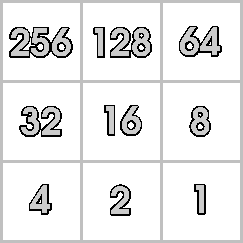
\includegraphics[scale=0.8]{appendices/map_rule_ordering.pdf}
		\caption{The index of a configuration is the sum of the numbers on its live cells.}
		\label{fig:map_rule_ordering_rule}
	\end{subfigure} \hfill \begin{subfigure}{.65\textwidth}
		\centering
		\patternimg{0.22}{map_rule_ordering_eg}
		\caption{From left to right, these are configurations (first row) $0$, $1$, $2$, $2+1=3$, (second row) $4$, $16+1=17$, $256+64+16+8+4=348$, and $256+128+64+32+16+8+4+2+1=511$.}
		\label{fig:map_rule_ordering_eg}
	\end{subfigure}
	\caption{To order the $2^9 = 512$ possible configurations of $3 \times 3$ live cells, we assign each one an index that is the sum of the numbers from~(a) that are on live cells. The ``0th'' configuration is thus the one with all cells dead, the ``1st'' configuration is the one with only the bottom-right cell alive, and so on.}\label{fig:map_rule_ordering}
\end{figure}

When ordering these configurations, we start counting as $0$ so that the all-dead configuration is the ``0th'' one (which is listed first), the configuration with only the bottom-right cell alive is the ``1st'' one (which is listed second), and so on. To create a rulestring for a non-isotropic CA, we now do two things:\smallskip

\begin{itemize}
	\item[1)] We create a 512-bit string of $0$s and $1$s that specifies which configurations (in the ordering specified by Figure~\ref{fig:map_rule_ordering}) lead to the central cell being dead or alive, respectively, in the next generation.
	
	For example, if cells are only born if they have no neighbors or a single neighbor to their southeast, and they only survive if they have neighbors everywhere \emph{except} for to their north and northwest,\footnote{This is the cellular automaton that was used by the knightship of Figure~\ref{fig:single_cell_knightship}.} then there are only three configurations of $3 \times 3$ grids of cells that lead to the central cell being alive in the next generation, and they correspond to indices $0$, $1$, and $64+32+16+8+4+2+1=127$. The $512$-bit string describing this rule thus has $1$s in its $0$th, $1$st, and $127$th locations, and $0$s elsewhere:
	\begin{align*}
		& \texttt{11000000 00000000 00000000 00000000 00000000 00000000 00000000 00000000} \\
		& \texttt{00000000 00000000 00000000 00000000 00000000 00000000 00000000 00000001} \\
		& \texttt{00000000 00000000 00000000 00000000 00000000 00000000 00000000 00000000} \\
		& \texttt{00000000 00000000 00000000 00000000 00000000 00000000 00000000 00000000} \\
		& \texttt{00000000 00000000 00000000 00000000 00000000 00000000 00000000 00000000} \\
		& \texttt{00000000 00000000 00000000 00000000 00000000 00000000 00000000 00000000} \\
		& \texttt{00000000 00000000 00000000 00000000 00000000 00000000 00000000 00000000} \\
		& \texttt{00000000 00000000 00000000 00000000 00000000 00000000 00000000 00000000}.
	\end{align*}
	
	\item[2)] In order to make the rule's description a bit shorter, we convert this 512-bit string from base~$2$ to base~$64$ according to Table~\ref{tab:base64}.\footnote{This is a fairly standard way of converting a bitstring to a mostly-alphanumeric string that shows up in lots of contexts outside of cellular automata as well.} Since each character in the base~$64$ string encodes $\log_2(64) = 6$ bits of the bitstring, this process gives a $\lceil 512/6 \rceil = 86$-character string that uniquely specifies the rule.\footnote{Since $512 \equiv 2 \ (\text{mod} \ 6)$, the final two bits of the bitstring correspond to the final character in the base-64 rulestring (and that character is determined by just the first two bits from Table~\ref{tab:base64}). This leads to some redundancy in the base-64 rulestrings: a final character of ``\texttt{A}'' indicates the same rule as a final character of ``\texttt{P}'', for example, and any of the final characters ``\texttt{g}'' through ``\texttt{v}'' are equivalent to each other.} Finally, we prepend this base-64 string with the characters ``\texttt{MAP}''\index{MAP} just to indicate that it is a non-isotropic rulestring.
	
	For example, if we convert the bitstring that we saw in part~(1) to base~$64$, the first 6 bits (``\texttt{110000}'') become ``\texttt{w}'', several groups of 6 bits (``\texttt{000000}'') each become ``\texttt{A}'', and one of the central groups of 6 bits (``\texttt{010000}'') becomes ``\texttt{Q}''. Altogether, the rulestring that describes this cellular automaton is
	\begin{align*}
		& \texttt{MAPwAAAAAAAAAAAAAAAAAAAAQAAAAAAAAAAAAAAAAAAAAA} \\
		& \texttt{\hphantom{MAP}AAAAAAAAAAAAAAAAAAAAAAAAAAAAAAAAAAAAAAAAAAA}.
	\end{align*}
\end{itemize}

\clearpage% for spacing reasons -- remove if layout changes

\begin{table}[!htb]
	\begin{center}		
		\begin{tabular}{cc|cc|cc|cc}
			\toprule
			Base $2$ & Base $64$ & Base $2$ & Base $64$ & Base $2$ & Base $64$ & Base $2$ & Base $64$ \\ \midrule
			\texttt{000000} & \texttt{A} & \texttt{010000} & \texttt{Q} & \texttt{100000} & \texttt{g} & \texttt{110000} & \texttt{w} \\
			\texttt{000001} & \texttt{B} & \texttt{010001} & \texttt{R} & \texttt{100001} & \texttt{h} & \texttt{110001} & \texttt{x} \\
			\texttt{000010} & \texttt{C} & \texttt{010010} & \texttt{S} & \texttt{100010} & \texttt{i} & \texttt{110010} & \texttt{y} \\
			\texttt{000011} & \texttt{D} & \texttt{010011} & \texttt{T} & \texttt{100011} & \texttt{j} & \texttt{110011} & \texttt{z} \\
			\texttt{000100} & \texttt{E} & \texttt{010100} & \texttt{U} & \texttt{100100} & \texttt{k} & \texttt{110100} & \texttt{0} \\
			\texttt{000101} & \texttt{F} & \texttt{010101} & \texttt{V} & \texttt{100101} & \texttt{l} & \texttt{110101} & \texttt{1} \\
			\texttt{000110} & \texttt{G} & \texttt{010110} & \texttt{W} & \texttt{100110} & \texttt{m} & \texttt{110110} & \texttt{2} \\
			\texttt{000111} & \texttt{H} & \texttt{010111} & \texttt{X} & \texttt{100111} & \texttt{n} & \texttt{110111} & \texttt{3} \\
			\texttt{001000} & \texttt{I} & \texttt{011000} & \texttt{Y} & \texttt{101000} & \texttt{o} & \texttt{111000} & \texttt{4} \\
			\texttt{001001} & \texttt{J} & \texttt{011001} & \texttt{Z} & \texttt{101001} & \texttt{p} & \texttt{111001} & \texttt{5} \\
			\texttt{001010} & \texttt{K} & \texttt{011010} & \texttt{a} & \texttt{101010} & \texttt{q} & \texttt{111010} & \texttt{6} \\
			\texttt{001011} & \texttt{L} & \texttt{011011} & \texttt{b} & \texttt{101011} & \texttt{r} & \texttt{111011} & \texttt{7} \\
			\texttt{001100} & \texttt{M} & \texttt{011100} & \texttt{c} & \texttt{101100} & \texttt{s} & \texttt{111100} & \texttt{8} \\
			\texttt{001101} & \texttt{N} & \texttt{011101} & \texttt{d} & \texttt{101101} & \texttt{t} & \texttt{111101} & \texttt{9} \\
			\texttt{001110} & \texttt{O} & \texttt{011110} & \texttt{e} & \texttt{101110} & \texttt{u} & \texttt{111110} & \texttt{+} \\
			\texttt{001111} & \texttt{P} & \texttt{011111} & \texttt{f} & \texttt{101111} & \texttt{v} & \texttt{111111} & \texttt{/} \\\bottomrule
		\end{tabular}
		\caption{A way of converting a (base-2) bitstring into a base-64 string. Every substring consisting of six bits gets mapped to a single alphanumeric character, or ``\texttt{+}'' or ``\texttt{/}''.}\label{tab:base64}
	\end{center}
\end{table}


%%%%%%%%%%%%%%%%%%%%%%%%%%%%%%%%
\section{\texorpdfstring{$\pi$}{Pi} Calculator APGsembly Code}\label{sec:appendix_apg}
%%%%%%%%%%%%%%%%%%%%%%%%%%%%%%%%

In Section~\ref{sec:pi_calc}, we developed an algorithm and pseudocode for computing the decimal digits of $\pi = 3.14159\ldots$. We now present the full APGsembly code that implements that algorithm and pseudocode, and was used to compile the $\pi$~calculator that we saw in Figure~\ref{fig:pi_calc}. In particular, APGsembly~\ref{alg:apgsembly_pi1} and~\ref{alg:apgsembly_pi2} implements that pseudocode via sliding block (unary) registers \texttt{U0}, \texttt{U1}, $\ldots$, \texttt{U9} and binary registers \texttt{B0}, \texttt{B1}, \texttt{B2}, \texttt{B3} that store the following quantities (the $A_n$ and $B_n$ matrices and quantities $q_n$ and $r_n$ are as defined in Section~\ref{sec:pi_calc}):\smallskip

\begin{itemize}
	\item[\texttt{U0}:] the top-left corner of the $A_n$ matrix
	
	\item[\texttt{U1}:] the top-right and bottom-right corners of the $A_n$ matrix
	
	\item[\texttt{U2}:] the current digit being computed
	
	\item[\texttt{U3}:] the index of the current digit (\texttt{U3}${} = 0$ for ``3'', \texttt{U3}${} = 1$ for ``1'', \texttt{U3}${} = 2$ for ``4'', and so on)
	
	\item[\texttt{U4}:] the number of times that the iteration has run, typically denoted here by $n$
	
	\item[\texttt{U5}:] counter that forces the program to iterate 4 times before printing a digit

	\item[\texttt{U6}:] the number of bits of memory allocated to the binary registers
	
	\item[\texttt{U7}--\texttt{U9}:] temporary registers used to help perform arithmetic operations and miscellaneous loops\smallskip
	
	\item[\texttt{B0}:] the top-left corner of the $B_n$ matrix
	
	\item[\texttt{B1}:] the top-right corner of the $B_n$ matrix ($= q_n$)
	
	\item[\texttt{B2}:] the bottom-right corner of the $B_n$ matrix ($= r_n$)
	
	\item[\texttt{B3}:] temporary register used to help perform arithmetic operations\smallskip
\end{itemize}

Recall that lines listed with a substate (input value) \texttt{*} just do the same actions and jump operation regardless of whether they receive a \texttt{Z} or \texttt{NZ} input value.

\begin{apgsembly}
	\centering
	\begin{minipage}[t]{.49\textwidth}
		\begin{algorithmic}\tiny
			\State \verb|#COMPONENTS NOP,OUTPUT,B0-3,U0-9,ADD,SUB,MUL|
			\State \verb|#REGISTERS {'U1':1, 'U6':6, 'B0':[0,'01']	, 'B2':[0,'1']}|
			\State \verb|# State    Input    Next state    Actions|
			\State \verb|# ---------------------------------------|
			\State \verb|INITIAL;   ZZ;      ITER1;        NOP|
			\State \verb||
			\State \verb|# Iterate 4 times per digit.|
			\State \verb|ITER1;     ZZ;      ITER2;        INC U5, NOP|
			\State \verb|ITER2;     ZZ;      ITER3;        INC U5, NOP|
			\State \verb|ITER3;     ZZ;      ITER4;        INC U5, NOP|
			\State \verb|ITER4;     ZZ;      ITER5;        INC U5, NOP|
			\State \verb|ITER5;     ZZ;      ITER6;        TDEC U5|
			\State \verb||
			\State \verb|# Each iteration, set U0 = U0 + 1, U1 = U1 + 2.|
			\State \verb|ITER6;     Z;       ITER11;       TDEC U3|
			\State \verb|ITER6;     NZ;      ITER7;        INC U0, INC U1, NOP|
			\State \verb|ITER7;     ZZ;      MULA1;        INC U1, NOP|
			\State \verb||
			\State \verb|## The MULA states set B3 = B1, B1 = U1 * B1.|
			\State \verb|# Copy B1 into B3, without erasing B1.|
			\State \verb|MULA1;     ZZ;      MULA2;        TDEC U6|
			\State \verb|MULA2;     Z;       MULA3;        TDEC U9|
			\State \verb|MULA2;     NZ;      MULA2;        TDEC U6, INC U9|
			\State \verb|MULA3;     Z;       MULA4;        TDEC U7|
			\State \verb|MULA3;     NZ;      MULA3;        TDEC U9, INC U6, INC U7|
			\State \verb|MULA4;     Z;       MULA8;        TDEC B1|
			\State \verb|MULA4;     NZ;      MULA5;        READ B1|
			\State \verb|MULA5;     Z;       MULA7;        READ B3|
			\State \verb|MULA5;     NZ;      MULA6;        SET B1, READ B3|
			\State \verb|MULA6;     *;       MULA7;        SET B3, NOP|
			\State \verb|MULA7;     *;       MULA4;        INC B1, INC B3, TDEC U7|
			\State \verb|MULA8;     Z;       MULA9;        TDEC B3|
			\State \verb|MULA8;     NZ;      MULA8;        TDEC B1|
			\State \verb|MULA9;     Z;       MULA10;       TDEC U1|
			\State \verb|MULA9;     NZ;      MULA9;        TDEC B3|
			\State \verb||
			\State \verb|# Copy U1 to temporary register U8.|
			\State \verb|MULA10;    Z;       MULA11;       TDEC U7|
			\State \verb|MULA10;    NZ;      MULA10;       TDEC U1, INC U7|
			\State \verb|MULA11;    Z;       MULA12;       TDEC U8|
			\State \verb|MULA11;    NZ;      MULA11;       TDEC U7, INC U1, INC U8|
			\State \verb||
			\State \verb|# Set B1 = U1 * B3 and U8 = 0.|
			\State \verb|MULA12;    *;       MULA13;       TDEC U8|
			\State \verb|MULA13;    Z;       MULB1;        TDEC U6|
			\State \verb|MULA13;    NZ;      MULA14;       TDEC U6|
			\State \verb|MULA14;    Z;       MULA15;       TDEC U9|
			\State \verb|MULA14;    NZ;      MULA14;       TDEC U6, INC U9|
			\State \verb|MULA15;    Z;       MULA16;       TDEC U7|
			\State \verb|MULA15;    NZ;      MULA15;       TDEC U9, INC U6, INC U7|
			\State \verb|MULA16;    Z;       MULA20;       TDEC B3|
			\State \verb|MULA16;    NZ;      MULA17;       READ B3|
			\State \verb|MULA17;    Z;       MULA18;       READ B1|
			\State \verb|MULA17;    NZ;      MULA18;       READ B1, SET B3, ADD A1|
			\State \verb|MULA18;    Z;       MULA19;       ADD B0|
			\State \verb|MULA18;    NZ;      MULA19;       ADD B1|
			\State \verb|MULA19;    Z;       MULA16;       TDEC U7, INC B1, INC B3|
			\State \verb|MULA19;    NZ;      MULA19;       SET B1, NOP|
			\State \verb|MULA20;    Z;       MULA21;       TDEC B1|
			\State \verb|MULA20;    NZ;      MULA20;       TDEC B3|
			\State \verb|MULA21;    Z;       MULA13;       TDEC U8|
			\State \verb|MULA21;    NZ;      MULA21;       TDEC B1|
			\State \verb||
			\State \verb|## The MULB states set B3 = B0, B0 = U0 * B0.|
			\State \verb|# Copy B0 into B3, without erasing B0.|
			\State \verb|MULB1;     Z;       MULB2;        TDEC U9|
			\State \verb|MULB1;     NZ;      MULB1;        TDEC U6, INC U9|
			\State \verb|MULB2;     Z;       MULB3;        TDEC U7|
			\State \verb|MULB2;     NZ;      MULB2;        TDEC U9, INC U6, INC U7|
			\State \verb|MULB3;     Z;       MULB6;        TDEC B0|
			\State \verb|MULB3;     NZ;      MULB4;        READ B3|
			\State \verb|MULB4;     *;       MULB5;        READ B0|
			\State \verb|MULB5;     Z;       MULB3;        INC B0, INC B3, TDEC U7|
			\State \verb|MULB5;     NZ;      MULB5;        SET B0, SET B3, NOP|
			\State \verb|MULB6;     Z;       MULB7;        TDEC B3|
			\State \verb|MULB6;     NZ;      MULB6;        TDEC B0|
			\State \verb|MULB7;     Z;       MULB8;        TDEC U0|
			\State \verb|MULB7;     NZ;      MULB7;        TDEC B3|
			\State \verb||
			\State \verb|# Copy U0 to temporary register U8.|
			\State \verb|MULB8;     Z;       MULB9;        TDEC U7|
			\State \verb|MULB8;     NZ;      MULB8;        TDEC U0, INC U7|
			\State \verb|MULB9;     Z;       MULB10;       TDEC U8|
			\State \verb|MULB9;     NZ;      MULB9;        TDEC U7, INC U0, INC U8|
		\end{algorithmic}
	\end{minipage}\hfill{\color{gray}\vline}\hfill
	\begin{minipage}[t]{.49\textwidth}
		\begin{algorithmic}\tiny
			\State \verb|# Set B0 = U0 * B3 and U8 = 0.|
			\State \verb|MULB10;    *;       MULB11;       TDEC U8|
			\State \verb|MULB11;    Z;       MULC1;        TDEC U1|
			\State \verb|MULB11;    NZ;      MULB12;       TDEC U6|
			\State \verb|MULB12;    Z;       MULB13;       TDEC U9|
			\State \verb|MULB12;    NZ;      MULB12;       TDEC U6, INC U9|
			\State \verb|MULB13;    Z;       MULB14;       TDEC U7|
			\State \verb|MULB13;    NZ;      MULB13;       TDEC U9, INC U6, INC U7|
			\State \verb|MULB14;    Z;       MULB18;       TDEC B3|
			\State \verb|MULB14;    NZ;      MULB15;       READ B3|
			\State \verb|MULB15;    Z;       MULB16;       READ B0|
			\State \verb|MULB15;    NZ;      MULB16;       READ B0, SET B3, ADD A1|
			\State \verb|MULB16;    Z;       MULB17;       ADD B0|
			\State \verb|MULB16;    NZ;      MULB17;       ADD B1|
			\State \verb|MULB17;    Z;       MULB14;       TDEC U7, INC B0, INC B3|
			\State \verb|MULB17;    NZ;      MULB17;       SET B0, NOP|
			\State \verb|MULB18;    Z;       MULB19;       TDEC B0|
			\State \verb|MULB18;    NZ;      MULB18;       TDEC B3|
			\State \verb|MULB19;    Z;       MULB11;       TDEC U8|
			\State \verb|MULB19;    NZ;      MULB19;       TDEC B0|
			\State \verb||
			\State \verb|## The MULC states set B1 = B1 + (U1 * B0).|
			\State \verb|# Copy U1 to temporary register U8.|
			\State \verb|MULC1;     Z;       MULC2;        TDEC U7|
			\State \verb|MULC1;     NZ;      MULC1;        TDEC U1, INC U7|
			\State \verb|MULC2;     Z;       MULC3;        TDEC U8|
			\State \verb|MULC2;     NZ;      MULC2;        TDEC U7, INC U1, INC U8|
			\State \verb||
			\State \verb|# Set B1 = B1 + (U1 * B3) and U8 = 0.|
			\State \verb|MULC3;     Z;       MULD1;        TDEC U6|
			\State \verb|MULC3;     NZ;      MULC4;        TDEC U6|
			\State \verb|MULC4;     Z;       MULC5;        TDEC U9|
			\State \verb|MULC4;     NZ;      MULC4;        TDEC U6, INC U9|
			\State \verb|MULC5;     Z;       MULC6;        TDEC U7|
			\State \verb|MULC5;     NZ;      MULC5;        TDEC U9, INC U6, INC U7|
			\State \verb|MULC6;     Z;       MULC10;       TDEC B3|
			\State \verb|MULC6;     NZ;      MULC7;        READ B3|
			\State \verb|MULC7;     Z;       MULC8;        READ B1|
			\State \verb|MULC7;     NZ;      MULC8;        READ B1, SET B3, ADD A1|
			\State \verb|MULC8;     Z;       MULC9;        ADD B0|
			\State \verb|MULC8;     NZ;      MULC9;        ADD B1|
			\State \verb|MULC9;     Z;       MULC6;        TDEC U7, INC B1, INC B3|
			\State \verb|MULC9;     NZ;      MULC9;        SET B1, NOP|
			\State \verb|MULC10;    Z;       MULC11;       TDEC B1|
			\State \verb|MULC10;    NZ;      MULC10;       TDEC B3|
			\State \verb|MULC11;    Z;       MULC3;        TDEC U8|
			\State \verb|MULC11;    NZ;      MULC11;       TDEC B1|
			\State \verb||
			\State \verb|## The MULD states set B2 = U1 * B2.|
			\State \verb|# Copy B2 into B3, without erasing B2.|
			\State \verb|MULD1;     Z;       MULD2;        TDEC U9|
			\State \verb|MULD1;     NZ;      MULD1;        TDEC U6, INC U9|
			\State \verb|MULD2;     Z;       MULD3;        TDEC U7|
			\State \verb|MULD2;     NZ;      MULD2;        TDEC U9, INC U6, INC U7|
			\State \verb|MULD3;     Z;       MULD6;        TDEC B2|
			\State \verb|MULD3;     NZ;      MULD4;        READ B3|
			\State \verb|MULD4;     *;       MULD5;        READ B2|
			\State \verb|MULD5;     Z;       MULD3;        INC B2, INC B3, TDEC U7|
			\State \verb|MULD5;     NZ;      MULD5;        SET B2, SET B3, NOP|
			\State \verb|MULD6;     Z;       MULD7;        TDEC B3|
			\State \verb|MULD6;     NZ;      MULD6;        TDEC B2|
			\State \verb|MULD7;     Z;       MULD8;        TDEC U1|
			\State \verb|MULD7;     NZ;      MULD7;        TDEC B3|
			\State \verb||
			\State \verb|# Copy U1 to temporary register U8.|
			\State \verb|MULD8;     Z;       MULD9;        TDEC U7|
			\State \verb|MULD8;     NZ;      MULD8;        TDEC U1, INC U7|
			\State \verb|MULD9;     Z;       MULD10;       TDEC U8|
			\State \verb|MULD9;     NZ;      MULD9;        TDEC U7, INC U1, INC U8|
			\State \verb||
			\State \verb|# Set B2 = U1 * B3 and U8 = 0.|
			\State \verb|MULD10;    *;       MULD11;       TDEC U8|
			\State \verb|MULD11;    Z;       ITER8;        INC U4, NOP|
			\State \verb|MULD11;    NZ;      MULD12;       TDEC U6|
			\State \verb|MULD12;    Z;       MULD13;       TDEC U9|
			\State \verb|MULD12;    NZ;      MULD12;       TDEC U6, INC U9|
			\State \verb|MULD13;    Z;       MULD14;       TDEC U7|
			\State \verb|MULD13;    NZ;      MULD13;       TDEC U9, INC U6, INC U7|
			\State \verb|MULD14;    Z;       MULD18;       TDEC B3|
			\State \verb|MULD14;    NZ;      MULD15;       READ B3|
			\State \verb|MULD15;    Z;       MULD16;       READ B2|
			\State \verb|MULD15;    NZ;      MULD16;       READ B2, SET B3, ADD A1|
			\State \verb|MULD16;    Z;       MULD17;       ADD B0|
			\State \verb|MULD16;    NZ;      MULD17;       ADD B1|
			\State \verb|MULD17;    Z;       MULD14;       INC B2, INC B3, TDEC U7|
			\State \verb|MULD17;    NZ;      MULD17;       SET B2, NOP|
			\State \verb|MULD18;    Z;       MULD19;       TDEC B2|
			\State \verb|MULD18;    NZ;      MULD18;       TDEC B3|
			\State \verb|MULD19;    Z;       MULD11;       TDEC U8|
			\State \verb|MULD19;    NZ;      MULD19;       TDEC B2|
		\end{algorithmic}
	\end{minipage}
	\caption{Page 1 of APGsembly code for a $\pi$ calculator that implements Pseudocode~\ref{alg:pseudocode_pi_calc}.}\label{alg:apgsembly_pi1}
\end{apgsembly}

\begin{apgsembly}
	\centering
	\begin{minipage}[t]{.49\textwidth}
		\begin{algorithmic}\tiny
			\State \verb|# Increase the amount of memory that we are allocating to the|
			\State \verb|# binary registers, by adding U4 to U6.|
			\State \verb|ITER8;     ZZ;      ITER9;        TDEC U4|
			\State \verb|ITER9;     Z;       ITER10;       TDEC U7|
			\State \verb|ITER9;     NZ;      ITER9;        TDEC U4, INC U7|
			\State \verb|ITER10;    Z;       ITER6;        TDEC U5|
			\State \verb|ITER10;    NZ;      ITER10;       TDEC U7, INC U4, INC U6|
			\State \verb||
			\State \verb|## Extract the units digit from (10^U3) * B1 / B2, as that is|
			\State \verb|## the digit of pi that we want to print.|
			\State \verb|# Copy U3 to temporary register U8.|
			\State \verb|ITER11;    Z;       ITER12;       TDEC U7|
			\State \verb|ITER11;    NZ;      ITER11;       TDEC U3, INC U7|
			\State \verb|ITER12;    Z;       ITER13;       TDEC U6|
			\State \verb|ITER12;    NZ;      ITER12;       TDEC U7, INC U3, INC U8|
			\State \verb||
			\State \verb|# Copy B1 into B3, without erasing B1.|
			\State \verb|ITER13;    Z;       ITER14;       TDEC U7|
			\State \verb|ITER13;    NZ;      ITER13;       TDEC U6, INC U7|
			\State \verb|ITER14;    Z;       ITER15;       TDEC U9|
			\State \verb|ITER14;    NZ;      ITER14;       TDEC U7, INC U6, INC U9|
			\State \verb|ITER15;    Z;       ITER18;       TDEC B3|
			\State \verb|ITER15;    NZ;      ITER16;       READ B3|
			\State \verb|ITER16;    *;       ITER17;       READ B1|
			\State \verb|ITER17;    Z;       ITER15;       INC B1, INC B3, TDEC U9|
			\State \verb|ITER17;    NZ;      ITER17;       SET B1, SET B3, NOP|
			\State \verb|ITER18;    Z;       ITER19;       TDEC B1|
			\State \verb|ITER18;    NZ;      ITER18;       TDEC B3|
			\State \verb|ITER19;    Z;       CMP1;         TDEC U6|
			\State \verb|ITER19;    NZ;      ITER19;       TDEC B1|
			\State \verb||
			\State \verb|# Now compare B2 with B3 to see which is bigger. This|
			\State \verb|# determines which of the two upcoming code blocks to go to.|
			\State \verb|CMP1;      Z;       CMP2;         TDEC U7|
			\State \verb|CMP1;      NZ;      CMP1;         TDEC U6, INC U7|
			\State \verb|CMP2;      Z;       CMP3;         TDEC U9|
			\State \verb|CMP2;      NZ;      CMP2;         TDEC U7, INC U6, INC U9|
			\State \verb|CMP3;      Z;       CMP4;         READ B3|
			\State \verb|CMP3;      NZ;      CMP3;         TDEC U9, INC B2, INC B3|
			\State \verb|CMP4;      Z;       CMP5;         READ B2|
			\State \verb|CMP4;      NZ;      CMP8;         READ B2, SET B3|
			\State \verb|CMP5;      Z;       CMP6;         TDEC B2|
			\State \verb|CMP5;      NZ;      CMP10;        TDEC B3, SET B2|
			\State \verb|CMP6;      *;       CMP7;         TDEC B3|
			\State \verb|CMP7;      Z;       CMP13;        TDEC B2|
			\State \verb|CMP7;      NZ;      CMP4;         READ B3|
			\State \verb|CMP8;      Z;       CMP12;        TDEC B3|
			\State \verb|CMP8;      NZ;      CMP9;         SET B2, NOP|
			\State \verb|CMP9;      ZZ;      CMP6;         TDEC B2|
			\State \verb|CMP10;     Z;       CMP11;        TDEC B2|
			\State \verb|CMP10;     NZ;      CMP10;        TDEC B3|
			\State \verb|CMP11;     Z;       DIG1;         TDEC U8|
			\State \verb|CMP11;     NZ;      CMP11;        TDEC B2|
			\State \verb|CMP12;     Z;       CMP13;        TDEC B2|
			\State \verb|CMP12;     NZ;      CMP12;        TDEC B3|
			\State \verb|CMP13;     Z;       SUB1;         TDEC U6|
			\State \verb|CMP13;     NZ;      CMP13;        TDEC B2|
			\State \verb||
			\State \verb|# If B2 <= B3 then subtract B2 from B3.|
			\State \verb|# That is, start or carry on with the integer division B3 / B2.|
			\State \verb|SUB1;      Z;       SUB2;         TDEC U7|
			\State \verb|SUB1;      NZ;      SUB1;         TDEC U6, INC U7|
			\State \verb|SUB2;      Z;       SUB3;         TDEC U9|
			\State \verb|SUB2;      NZ;      SUB2;         TDEC U7, INC U6, INC U9|
			\State \verb|SUB3;      Z;       SUB7;         TDEC B3|
			\State \verb|SUB3;      NZ;      SUB4;         READ B3|
			\State \verb|SUB4;      Z;       SUB5;         READ B2|
			\State \verb|SUB4;      NZ;      SUB5;         READ B2, SUB A1|
			\State \verb|SUB5;      Z;       SUB6;         SUB B0|
			\State \verb|SUB5;      NZ;      SUB6;         SUB B1, SET B2|
			\State \verb|SUB6;      Z;       SUB3;         INC B2, INC B3, TDEC U9|
			\State \verb|SUB6;      NZ;      SUB6;         SET B3, NOP|
			\State \verb|SUB7;      Z;       SUB8;         TDEC B2|
			\State \verb|SUB7;      NZ;      SUB7;         TDEC B3|
			\State \verb|SUB8;      Z;       CMP1;         TDEC U6, INC U2|
			\State \verb|SUB8;      NZ;      SUB8;         TDEC B2|
			\State \verb||
			\State \verb|# If B2 > B3 we cannot subtract anymore.|
			\State \verb|# Multiply B3 by 10 and reset U2, or jump ahead and print|
			\State \verb|# the digit that we have now computed.|
			\State \verb|DIG1;      Z;       OUT0;         TDEC U2|
			\State \verb|DIG1;      NZ;      DIG2;         TDEC U2|
			\State \verb|DIG2;      Z;       DIG3;         TDEC U6|
			\State \verb|DIG2;      NZ;      DIG2;         TDEC U2|
			\State \verb|DIG3;      Z;       DIG4;         TDEC U7|
			\State \verb|DIG3;      NZ;      DIG3;         TDEC U6, INC U7|
			\State \verb|DIG4;      Z;       DIG5;         TDEC U9|
			\State \verb|DIG4;      NZ;      DIG4;         TDEC U7, INC U6, INC U9|
			\State \verb|DIG5;      Z;       DIG8;         TDEC B3|
			\State \verb|DIG5;      NZ;      DIG6;         READ B3|
			\State \verb|DIG6;      Z;       DIG7;         MUL 0|
			\State \verb|DIG6;      NZ;      DIG7;         MUL 1|
			\State \verb|DIG7;      Z;       DIG5;         INC B3, TDEC U9|
			\State \verb|DIG7;      NZ;      DIG7;         SET B3, NOP|
			\State \verb|DIG8;      Z;       CMP1;         TDEC U6|
			\State \verb|DIG8;      NZ;      DIG8;         TDEC B3|
		\end{algorithmic}
	\end{minipage}\hfill{\color{gray}\vline}\hfill
	\begin{minipage}[t]{.49\textwidth}
		\begin{algorithmic}\tiny
			\State \verb|# Print the current digit, which is stored in U2.|
			\State \verb|OUT0;      Z;       OUTD1;        NOP, OUTPUT 0|
			\State \verb|OUT0;      NZ;      OUT1;         TDEC U2|
			\State \verb|OUT1;      Z;       OUTD1;        NOP, OUTPUT 1|
			\State \verb|OUT1;      NZ;      OUT2;         TDEC U2|
			\State \verb|OUT2;      Z;       OUTD1;        NOP, OUTPUT 2|
			\State \verb|OUT2;      NZ;      OUT3;         TDEC U2|
			\State \verb|OUT3;      Z;       OUTD1;        NOP, OUTPUT 3|
			\State \verb|OUT3;      NZ;      OUT4;         TDEC U2|
			\State \verb|OUT4;      Z;       OUTD1;        NOP, OUTPUT 4|
			\State \verb|OUT4;      NZ;      OUT5;         TDEC U2|
			\State \verb|OUT5;      Z;       OUTD1;        NOP, OUTPUT 5|
			\State \verb|OUT5;      NZ;      OUT6;         TDEC U2|
			\State \verb|OUT6;      Z;       OUTD1;        NOP, OUTPUT 6|
			\State \verb|OUT6;      NZ;      OUT7;         TDEC U2|
			\State \verb|OUT7;      Z;       OUTD1;        NOP, OUTPUT 7|
			\State \verb|OUT7;      NZ;      OUT8;         TDEC U2|
			\State \verb|OUT8;      Z;       OUTD1;        NOP, OUTPUT 8|
			\State \verb|OUT8;      NZ;      OUTD1;        NOP, OUTPUT 9|
			\State \verb||
			\State \verb|# Check whether or not we just printed the very first digit (3).|
			\State \verb|# If so, print a decimal point. Either way, increase U3, which|
			\State \verb|# counts which decimal place we are currently at, and loop back|
			\State \verb|# to start the next digit calculation.|
			\State \verb|OUTD1;     ZZ;      OUTD2;        TDEC U3|
			\State \verb|OUTD2;     Z;       ITER1;        INC U3, NOP, OUTPUT .|
			\State \verb|OUTD2;     NZ;      OUTD3;        INC U3, NOP|
			\State \verb|OUTD3;     ZZ;      ITER1;        INC U3, NOP|
		\end{algorithmic}
	\end{minipage}
	\caption{Page 2 of APGsembly code for a $\pi$ calculator that implements Pseudocode~\ref{alg:pseudocode_pi_calc}.}\label{alg:apgsembly_pi2}
\end{apgsembly}